\documentclass[10pt,openany]{book}
\usepackage{iftex}
\ifPDFTeX
\usepackage[utf8]{inputenc}
\DeclareUnicodeCharacter{2212}{\ensuremath{-}}
\DeclareUnicodeCharacter{2192}{\ensuremath{\to}}
\DeclareUnicodeCharacter{03B1}{\ensuremath{\alpha}}
\DeclareUnicodeCharacter{2248}{\ensuremath{\approx}}
\DeclareUnicodeCharacter{00D7}{\ensuremath{\times}}
\DeclareUnicodeCharacter{0394}{\ensuremath{\Delta}}
\DeclareUnicodeCharacter{2074}{\ensuremath{^4}}
\fi
\usepackage[T1]{fontenc}
\usepackage{lmodern}
\AtBeginDocument{\normalfont\DeclareFontShape{T1}{lmr}{bx}{sc}{<->ssub*lmr/m/sc}{}}
\usepackage[spanish,es-nodecimaldot]{babel}
\spanishplainpercent
\AtBeginDocument{\spanishdeactivate{"~<>}}
\usepackage[a4paper,margin=2.5cm,headheight=14pt]{geometry}
\usepackage{needspace}
\usepackage{amsmath,amssymb,mathtools,booktabs,array,longtable,graphicx,xcolor,tikz,enumitem,microtype,titlesec,fancyhdr}
\usepackage[breakable,skins]{tcolorbox}
\usepackage[labelfont=bf]{caption}
\usepackage[hyphens]{url}
\usepackage[hidelinks,unicode,hypertexnames=false]{hyperref}
\definecolor{studiumInk}{RGB}{20,44,64}
\definecolor{studiumBlue}{RGB}{24,74,130}
\definecolor{studiumCyan}{RGB}{0,184,205}
\definecolor{studiumLight}{RGB}{232,240,250}
\definecolor{studiumWorkedBack}{RGB}{255,244,230}
\definecolor{studiumWorkedFrame}{RGB}{138,78,12}
\definecolor{studiumCheckBack}{RGB}{243,236,248}
\definecolor{studiumCheckFrame}{RGB}{96,48,130}
\titleformat{\chapter}[display]{\normalfont\filright}{\large\mdseries\scshape\chaptertitlename\ \thechapter}{1ex}{\normalfont\huge\bfseries}
\titlespacing*{\chapter}{0pt}{2.5ex plus 1ex minus .2ex}{2.3ex}
\titleformat{name=\chapter,numberless}[display]{\normalfont\filright}{}{0pt}{\normalfont\huge\bfseries}
\titleformat{\section}{\Large\bfseries}{\thesection}{.8em}{}
\titleformat{\subsection}{\large\bfseries}{\thesubsection}{.7em}{}
\makeatletter
\renewcommand*\l@section{\@dottedtocline{1}{1.5em}{3.5em}}
\renewcommand*\l@subsection{\@dottedtocline{2}{3.8em}{5em}}
\makeatother
\setcounter{secnumdepth}{2}\setcounter{tocdepth}{2}
\setlength{\parindent}{1.5em}\setlength{\parskip}{3pt plus .5pt}
\setlength{\emergencystretch}{1.5em}\raggedbottom
\setlist{itemsep=2pt,topsep=4pt,leftmargin=*}
\setlist[description]{style=nextline,leftmargin=0pt,labelwidth=0pt,labelindent=0pt}
\allowdisplaybreaks[2]
\graphicspath{{figures/}}
\newcommand{\Raire}{287.05287}
\newcommand{\gzero}{9.80665}
\tcbset{studiumcommon/.style={breakable,boxrule=.65pt,arc=.7pt,left=1.7mm,right=1.7mm,top=1.3mm,bottom=1.3mm,before skip=10pt,after skip=10pt,fonttitle=\bfseries}}
\newtcolorbox{studiumworked}[1]{studiumcommon,colback=studiumWorkedBack,colframe=studiumWorkedFrame,colbacktitle=studiumWorkedFrame,coltitle=white,title={#1}}
\newcommand{\objetivos}[1]{\par\noindent\textbf{Objetivos de aprendizaje.} \textit{#1}\par\medskip}
\newcommand{\caja}[2]{\begin{tcolorbox}[studiumcommon,colback=studiumLight,colframe=studiumBlue,colbacktitle=studiumBlue,coltitle=white,title={#1}]#2\end{tcolorbox}}
\newcommand{\resumen}[1]{\begin{tcolorbox}[studiumcommon,colback=studiumCheckBack,colframe=studiumCheckFrame,colbacktitle=studiumCheckFrame,coltitle=white,title=Resumen]#1\end{tcolorbox}}
\newcommand{\figura}[2]{\begin{figure}[tbp]\centering\includegraphics[width=.83\linewidth]{#1.pdf}\caption{#2}\label{fig:#1}\end{figure}\noindent La figura~\ref{fig:#1} ofrece una representación del modelo discutido.}
\pagestyle{fancy}\fancyhf{}
\fancyhead[LE]{\small\thepage\hspace{1.5em}\mdseries\scshape\nouppercase{\leftmark}}
\fancyhead[RO]{\small\mdseries\scshape\nouppercase{\rightmark}\hspace{1.5em}\thepage}
\renewcommand{\headrulewidth}{.4pt}\renewcommand{\footrulewidth}{0pt}
\fancypagestyle{plain}{\fancyhf{}\fancyfoot[C]{\small\thepage}\renewcommand{\headrulewidth}{0pt}}

% Retícula Studium unificada: cabecera blanca, fotografía a sangre y bloque azul.
\addto\captionsspanish{\renewcommand{\contentsname}{Índice}\renewcommand{\tablename}{Cuadro}\renewcommand{\listtablename}{Índice de cuadros}}
\numberwithin{equation}{chapter}
\let\cleardoublepage\clearpage
\fancyfoot[R]{\scriptsize\sffamily\color{studiumInk}En revisión}
\renewcommand{\chaptermark}[1]{\markboth{Capítulo \thechapter.\ #1}{}}
\renewcommand{\sectionmark}[1]{\markright{\thesection\ #1}}
\definecolor{studiumTipBack}{RGB}{232,244,236}
\definecolor{studiumTipFrame}{RGB}{27,107,58}
\newcommand{\consejo}[2]{\begin{tcolorbox}[studiumcommon,colback=studiumTipBack,colframe=studiumTipFrame,colbacktitle=studiumTipFrame,coltitle=white,title={#1}]#2\end{tcolorbox}}
\newcommand{\estado}{Edición íntegra de estudio. Pendiente de revisión experta independiente.}
\newcommand{\portada}[3]{%
\hypersetup{pageanchor=false}
\begin{titlepage}\thispagestyle{empty}
\begin{tikzpicture}[remember picture,overlay,x=1bp,y=-1bp]
\begin{scope}[shift={(current page.north west)}]
\clip (0,0) rectangle (595.276,841.89);
\fill[white] (0,0) rectangle (595.276,841.89);
% Hero fotografico preencuadrado en la reticula de la coleccion (mismo
% borde superior y mismo bloque inferior que Teoria de Estructuras/Fluidos).
\node[anchor=north west,inner sep=0pt,outer sep=0pt] at (0,89.5)
  {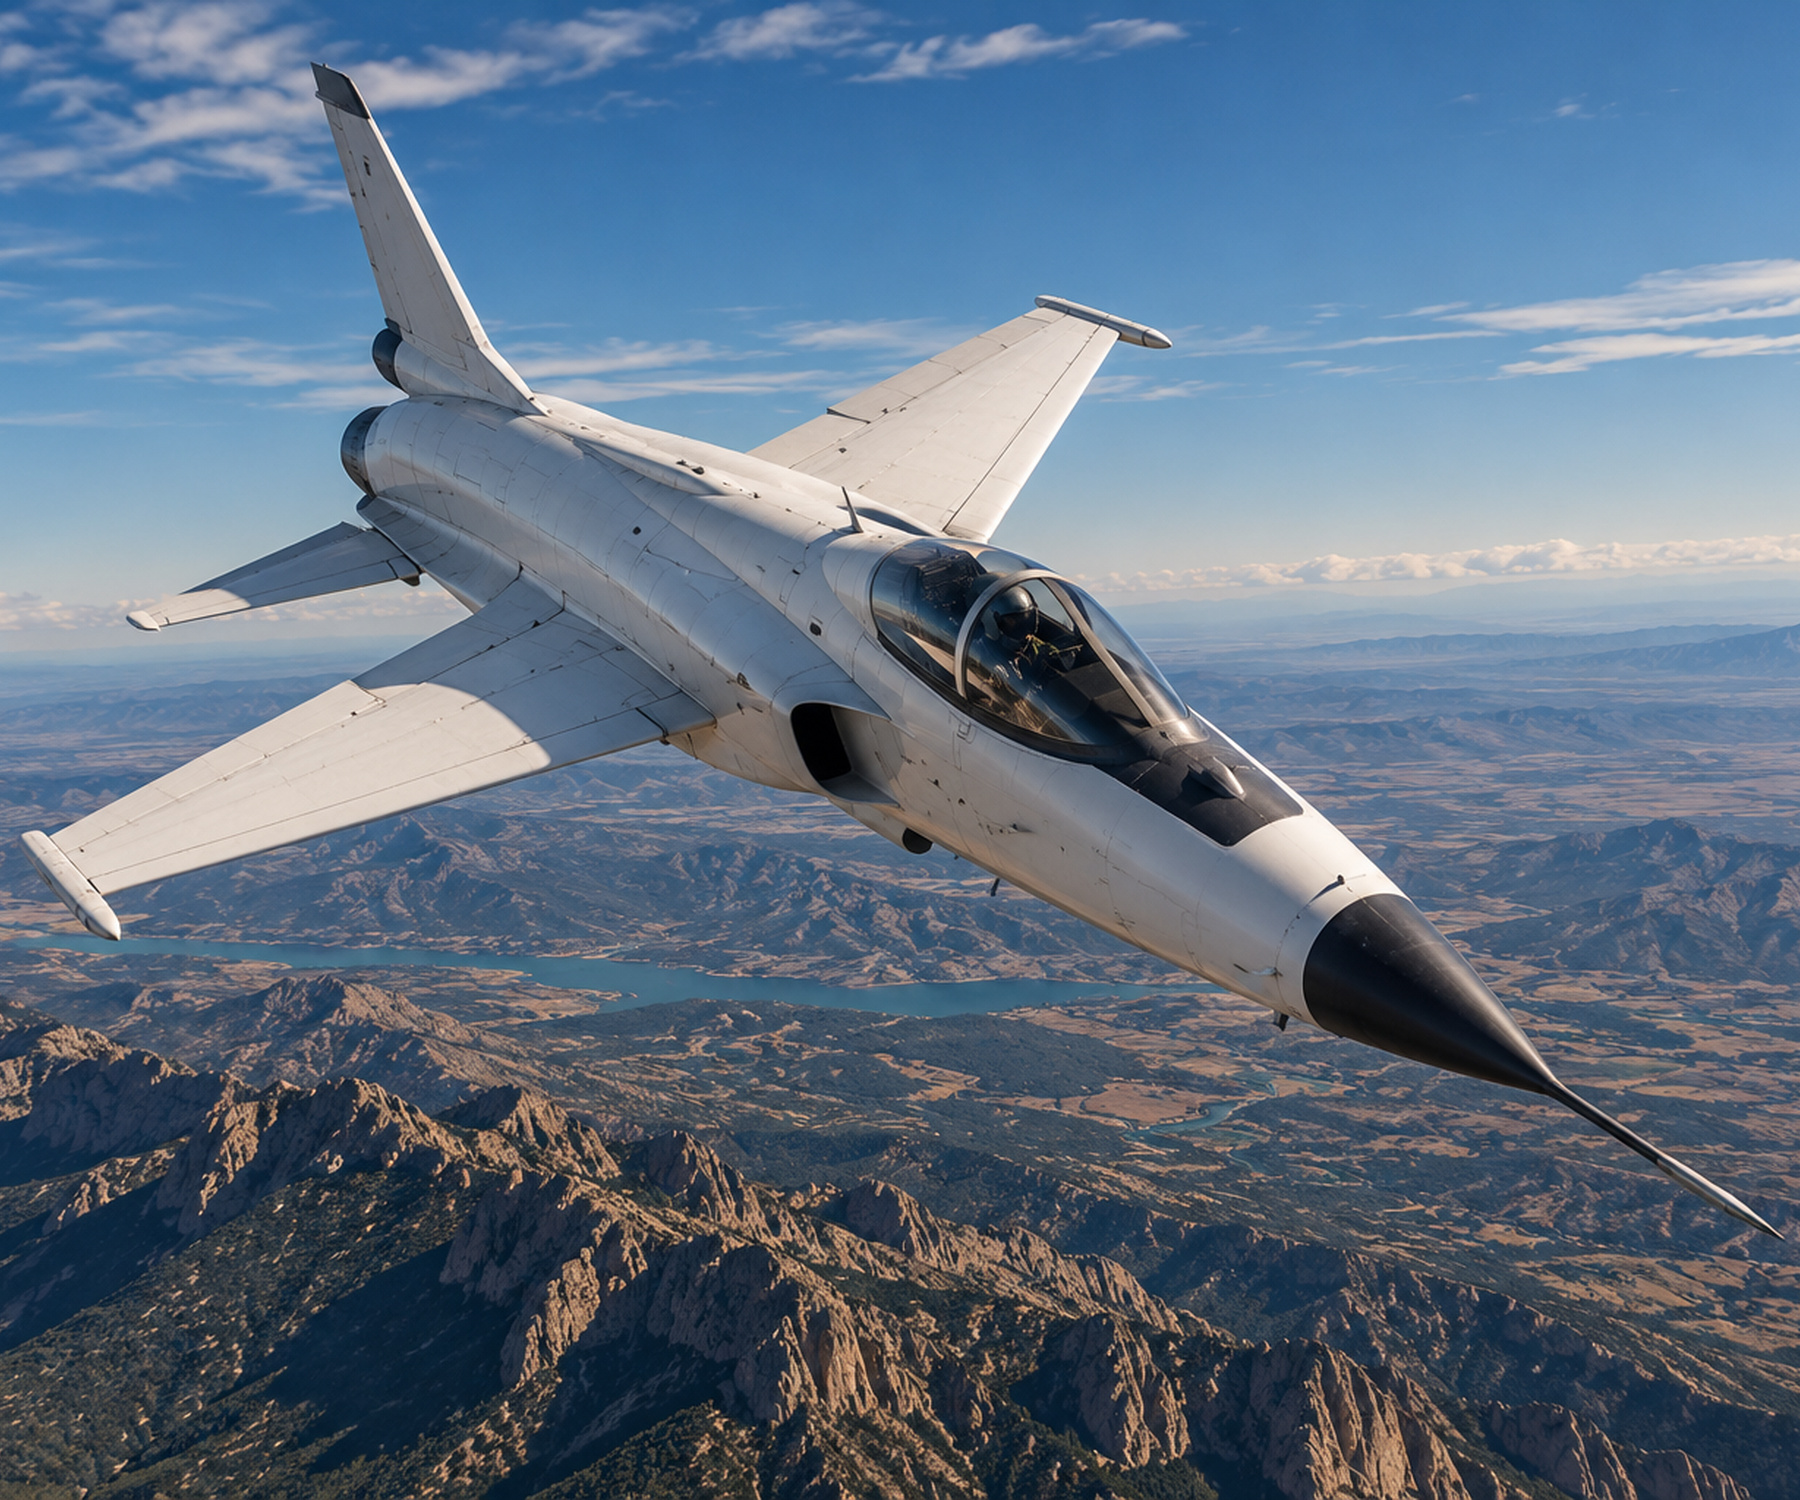
\includegraphics[width=595.276bp,height=496bp]{assets/cover-hero.jpg}};
\fill[studiumInk] (0,585.5) rectangle (595.276,841.89);
% Cabecera editorial.
% Logotipo auténtico de Studium: símbolo y letras extraídos sin redibujarlos
% de framework/docs/assets/studium-logo-dark.png, adaptados a una firma horizontal.
\node[anchor=north west,inner sep=0pt,outer sep=0pt] at (43,5)
  {
\includegraphics[width=185bp]{assets/studium-horizontal.png}};
\fill[studiumCyan] (106,76) rectangle (132,78);
\node[anchor=west,text=studiumInk,font=\sffamily\fontsize{8.2}{10}\selectfont,inner sep=0pt] at (140,79){BIBLIOTECA DE INGENIERÍA};
% Bloque inferior: tipografia, blancos y posiciones de la coleccion.
\node[anchor=west,text=studiumCyan,font=\sffamily\bfseries\fontsize{10}{12}\selectfont,inner sep=0pt] at (51.223,608){#1};
\node[anchor=north west,text=white,text width=493pt,font=\rmfamily\bfseries\fontsize{26.5}{29.5}\selectfont,inner sep=0pt] at (51.223,627){#2};
\node[anchor=north west,text=white!82!studiumInk,text width=493pt,font=\sffamily\fontsize{10}{13}\selectfont,inner sep=0pt] at (51.223,730){#3};
\node[anchor=west,text=white,font=\sffamily\bfseries\fontsize{10}{12}\selectfont,inner sep=0pt] at (51.223,774){GRADO EN INGENIERÍA AEROESPACIAL};
\node[anchor=west,text=white!82!studiumInk,font=\sffamily\fontsize{10}{12}\selectfont,inner sep=0pt] at (51.223,789){Universidad de León};
\draw[white!75!studiumInk,line width=.4pt] (51.223,801) -- (544.05,801);
\node[anchor=west,text=white!82!studiumInk,font=\sffamily\fontsize{10}{12}\selectfont,inner sep=0pt] at (51.223,822){2026};
\node[anchor=east,text=white,font=\sffamily\bfseries\fontsize{10}{12}\selectfont,inner sep=0pt] at (544.05,822){Primera edición};
\end{scope}\end{tikzpicture}\null
\end{titlepage}\hypersetup{pageanchor=true}}

\newcommand{\caso}[2]{\begin{studiumworked}{#1}#2\end{studiumworked}}
\newcommand{\ilustra}[2]{\begin{figure}[htbp]\centering\includegraphics[width=.94\linewidth]{#1.pdf}\caption{#2}\label{fig:#1}\end{figure}}
\newcommand{\fuentes}[1]{\par\medskip\noindent{\footnotesize\textbf{Fuentes y localizadores.} #1}\par}
\newcommand{\apartado}[2]{\par\medskip\noindent\textbf{#1.} #2\par}
\newcommand{\repaso}[2]{\par\medskip\noindent\textbf{Para comprobar la comprensión.} #1\par\noindent\textit{Respuesta razonada.} #2\par}

\newcommand{\vect}[1]{\boldsymbol{#1}}
\newcommand{\dd}{\mathrm{d}}
\newcommand{\SIu}[1]{\,\mathrm{#1}}
\newcommand{\hipotesis}[1]{\caja{Hipótesis y dominio}{#1}}
\newcommand{\verifica}[1]{\consejo{Comprobación y límites}{#1}}
\newcommand{\errorcomun}[1]{\caja{Error que cambia el resultado}{#1}}

\hypersetup{pdftitle={Problemas resueltos de Mecánica de Vuelo},pdfauthor={Studium}}
\begin{document}
\portada{CUADERNO DE PROBLEMAS}{PROBLEMAS RESUELTOS\\DE MECÁNICA DE VUELO}{Colección original · Fundamentos, actuaciones y estabilidad}
\frontmatter
\chapter*{Cómo usar la colección}
Esta colección contiene 43 problemas originales con datos docentes. Se distribuye en niveles básico, intermedio, avanzado y de examen. Cada solución declara sistema de referencia, hipótesis, ecuaciones, desarrollo, resultados, comprobación y límites. Los ejercicios no son exámenes oficiales ni soluciones de las prácticas evaluables facilitadas.

La comprobación propuesta puede utilizar un balance, un límite, una cuadratura o un método numérico distinto. Cuando una magnitud procede de una raíz u optimización, reproducir su literal no verifica el algoritmo: se conserva esa distinción en el registro. La revisión experta independiente permanece pendiente.
\par\smallskip
% Copyright / artwork statement for the image actually embedded in all PDFs.
\noindent\textbf{Imagen de portada.} Ilustración aeronáutica fotorrealista,
original y generada digitalmente para esta edición independiente de Studium
(2026). Representa una aeronave en maniobra de alabeo sobre un paisaje
montañoso; no es una fotografía documental ni representa un avión concreto.
El diseño incorpora el logotipo original de Studium proporcionado con el
proyecto. No implica aval de la Universidad de León ni de ninguna institución.

\tableofcontents
\mainmatter
\chapter{Básico}

\section{P01 · Consumo másico y ponderal}

\noindent\textbf{Nivel:} Básico.

\apartado{1. Enunciado}{Un reactor entrega $38\,000\SIu N$ con consumo específico $18.2\SIu{g/(kN\,s)}$. Obtenga gasto másico, consumo en 25 minutos y consumo ponderal equivalente.}

\apartado{2. Datos}{$T=38\,000\SIu N$, $c_T=18.2\times10^{-6}\SIu{kg/(N\,s)}$, $t=1500\SIu s$.}

\apartado{3. Incógnitas}{Gasto, masa consumida y consumo ponderal.}

\apartado{4. Sistema de referencia}{Escalares propulsivos; empuje en dirección de vuelo.}

\apartado{5. Hipótesis físicas}{Empuje y consumo específico constantes durante el intervalo.}

\apartado{6. Modelo matemático}{Gasto referido a empuje}

\apartado{7. Ecuaciones simbólicas}{Se parte de los balances y definiciones siguientes.}

\begin{equation}\dot m_f=c_TT\end{equation}

\begin{equation}\Delta m=\dot m_ft\end{equation}

\begin{equation}\widetilde c_T=g_0c_T\end{equation}

\apartado{8. Desarrollo algebraico}{Las operaciones se realizan en este orden, conservando las condiciones del modelo.}

\begin{enumerate}

\item Se convierten gramos a kg y kN a N: cada conversión aporta un factor de mil en sentidos distintos.

\item El gasto se multiplica por segundos, sin introducir gravedad en una masa.

\item El factor de gravedad se aplica sólo para pasar a consumo ponderal.

\end{enumerate}

\apartado{9. Sustitución numérica}{Se usan las magnitudes del apartado de datos en SI; los ángulos se convierten a radianes antes de evaluar funciones trigonométricas. Las densidades indicadas como ISA se obtienen de la capa correspondiente.}

\noindent Gasto:\quad $1.82 \cdot 10^{-5} \cdot 38000\simeq 0.6916\,\mathrm{kg\,s^{-1}}$.\par

\noindent Combustible:\quad $1.82 \cdot 10^{-5} \cdot 38000 \cdot 1500\simeq 1037.4\,\mathrm{kg}$.\par

\noindent Consumo ponderal:\quad $9.80665 \cdot 1.82 \cdot 10^{-5}\simeq 0.000178481\,\mathrm{s^{-1}}$.\par

\apartado{10. Resultados con unidades}{Los resultados pertenecen al modelo y al intervalo de datos declarados.}

\begin{center}\begin{tabular}{lr}\toprule Magnitud&Resultado\\\midrule

Gasto & $0.6916\,\mathrm{kg\,s^{-1}}$\\

Combustible & $1037.4\,\mathrm{kg}$\\

Consumo ponderal & $0.000178481\,\mathrm{s^{-1}}$\\

\bottomrule\end{tabular}\end{center}

\apartado{11. Interpretación}{El gasto constante no implica que el avión conserve masa; la masa del avión disminuye exactamente en la cantidad calculada.}

\apartado{12. Comprobación independiente y alcance}{Rehacer la operación en g/s: 18.2 g por kN y segundo multiplicados por 38 kN; convertir al final.}

\apartado{13. Limitaciones}{No se ha supuesto un mapa de motor válido fuera del intervalo.}

\par\smallskip\noindent{\footnotesize\textit{Datos y solución originales. Las sustituciones registradas se reproducen con SymPy y Studium; eso no establece validación experimental ni revisión experta.}}


\section{P02 · Velocidad en ejes cuerpo}

\noindent\textbf{Nivel:} Básico.

\apartado{1. Enunciado}{Una velocidad aérea tiene componentes cuerpo $(74,6,9)\SIu{m\,s^{-1}}$. Determine TAS, incidencia y resbalamiento y reconstruya el vector.}

\apartado{2. Datos}{$u_a=74$, $v_a=6$, $w_a=9$, en $\mathrm{m/s}$.}

\apartado{3. Incógnitas}{TAS, alpha y beta.}

\apartado{4. Sistema de referencia}{Cuerpo: x adelante, y derecha, z abajo; matriz pasiva viento a cuerpo.}

\apartado{5. Hipótesis físicas}{Velocidad no nula; ángulos dentro de la rama habitual de vuelo hacia delante.}

\apartado{6. Modelo matemático}{Definición de ángulos aerodinámicos}

\apartado{7. Ecuaciones simbólicas}{Se parte de los balances y definiciones siguientes.}

\begin{equation}V=\sqrt{u_a^2+v_a^2+w_a^2}\end{equation}

\begin{equation}\alpha=\arctan(w_a/u_a),\quad\beta=\arcsin(v_a/V)\end{equation}

\begin{equation}\vect v_a^b=V(\cos\alpha\cos\beta,\sin\beta,\sin\alpha\cos\beta)^T\end{equation}

\apartado{8. Desarrollo algebraico}{Las operaciones se realizan en este orden, conservando las condiciones del modelo.}

\begin{enumerate}

\item Se calcula primero el módulo de las tres componentes.

\item La incidencia utiliza w/u; el resbalamiento utiliza v/V y no v/u.

\item Los resultados angulares se convierten a grados sólo para presentación.

\end{enumerate}

\apartado{9. Sustitución numérica}{Se usan las magnitudes del apartado de datos en SI; los ángulos se convierten a radianes antes de evaluar funciones trigonométricas. Las densidades indicadas como ISA se obtienen de la capa correspondiente.}

\noindent TAS:\quad $\sqrt{6^{2} + 9^{2} + 74^{2}}\simeq 74.78636\,\mathrm{m\,s^{-1}}$.\par

\noindent Incidencia grados:\quad $\operatorname{atan}{\left(\frac{9}{74} \right)} 180 \frac{1}{\pi}\simeq 6.934349\,{}^\circ$.\par

\noindent Resbalamiento grados:\quad $\operatorname{asin}{\left(\frac{6}{\sqrt{6^{2} + 9^{2} + 74^{2}}} \right)} 180 \frac{1}{\pi}\simeq 4.601702\,{}^\circ$.\par

\apartado{10. Resultados con unidades}{Los resultados pertenecen al modelo y al intervalo de datos declarados.}

\begin{center}\begin{tabular}{lr}\toprule Magnitud&Resultado\\\midrule

TAS & $74.78636\,\mathrm{m\,s^{-1}}$\\

Incidencia grados & $6.934349\,{}^\circ$\\

Resbalamiento grados & $4.601702\,{}^\circ$\\

\bottomrule\end{tabular}\end{center}

\apartado{11. Interpretación}{El w positivo representa velocidad hacia abajo en cuerpo, sin determinar todavía ascenso o descenso terrestre.}

\apartado{12. Comprobación independiente y alcance}{Multiplicar V por la primera columna de Cbw y comprobar que recupera las tres entradas y su norma.}

\apartado{13. Limitaciones}{No hay información de actitud ni viento para reconstruir la trayectoria terrestre.}

\par\smallskip\noindent{\footnotesize\textit{Datos y solución originales. Las sustituciones registradas se reproducen con SymPy y Studium; eso no establece validación experimental ni revisión experta.}}


\section{P03 · Peso en actitud inclinada}

\noindent\textbf{Nivel:} Básico.

\apartado{1. Enunciado}{Un avión de $1800\SIu{kg}$ tiene alabeo $22^\circ$ y cabeceo $7^\circ$. Exprese el peso en cuerpo y compruebe su norma.}

\apartado{2. Datos}{$m=1800\SIu{kg}$, $\phi=22^\circ$, $\theta=7^\circ$.}

\apartado{3. Incógnitas}{Tres componentes de peso.}

\apartado{4. Sistema de referencia}{NED a cuerpo con Euler 3--2--1.}

\apartado{5. Hipótesis físicas}{Gravedad uniforme; no se necesitan guiñada ni velocidad para esta proyección.}

\apartado{6. Modelo matemático}{Transformación de gravedad}

\apartado{7. Ecuaciones simbólicas}{Se parte de los balances y definiciones siguientes.}

\begin{equation}\vect W^b=mg_0(-\sin\theta,\sin\phi\cos\theta,\cos\phi\cos\theta)^T\end{equation}

\apartado{8. Desarrollo algebraico}{Las operaciones se realizan en este orden, conservando las condiciones del modelo.}

\begin{enumerate}

\item Se transforman grados a radianes en las funciones trigonométricas.

\item El componente x es negativo con morro alto.

\item Los componentes y y z dependen del alabeo y del coseno de cabeceo.

\end{enumerate}

\apartado{9. Sustitución numérica}{Se usan las magnitudes del apartado de datos en SI; los ángulos se convierten a radianes antes de evaluar funciones trigonométricas. Las densidades indicadas como ISA se obtienen de la capa correspondiente.}

\noindent Wx:\quad $\left(-1800\right) 9.80665 \sin{\left(\frac{7 \pi}{180} \right)}\simeq -2151.234\,\mathrm N$.\par

\noindent Wy:\quad $1800 \cdot 9.80665 \sin{\left(\frac{22 \pi}{180} \right)} \cos{\left(\frac{7 \pi}{180} \right)}\simeq 6563.255\,\mathrm N$.\par

\noindent Wz:\quad $1800 \cdot 9.80665 \cos{\left(\frac{22 \pi}{180} \right)} \cos{\left(\frac{7 \pi}{180} \right)}\simeq 16244.63\,\mathrm N$.\par

\apartado{10. Resultados con unidades}{Los resultados pertenecen al modelo y al intervalo de datos declarados.}

\begin{center}\begin{tabular}{lr}\toprule Magnitud&Resultado\\\midrule

Wx & $-2151.234\,\mathrm N$\\

Wy & $6563.255\,\mathrm N$\\

Wz & $16244.63\,\mathrm N$\\

\bottomrule\end{tabular}\end{center}

\apartado{11. Interpretación}{La proyección lateral del peso no constituye por sí sola una fuerza aerodinámica lateral.}

\apartado{12. Comprobación independiente y alcance}{Usar ortogonalidad: la suma de cuadrados debe ser $ (mg_0)^2 $ y el límite $\phi=\theta=0$ debe dar sólo Wz.}

\apartado{13. Limitaciones}{No se añaden términos centrífugos a una gravedad ya definida como efectiva.}

\par\smallskip\noindent{\footnotesize\textit{Datos y solución originales. Las sustituciones registradas se reproducen con SymPy y Studium; eso no establece validación experimental ni revisión experta.}}


\section{P04 · Ruta con viento cruzado}

\noindent\textbf{Nivel:} Básico.

\apartado{1. Enunciado}{Una aeronave debe seguir una ruta este con TAS $68\SIu{m/s}$. El viento sopla hacia el norte a $16\SIu{m/s}$ y hacia el este a $5\SIu{m/s}$. Calcule corrección de rumbo y tiempo para $240\SIu{km}$.}

\apartado{2. Datos}{$V=68$, $U_\perp=16$, $U_\parallel=5$, en m/s; $R_g=240\,000\SIu m$.}

\apartado{3. Incógnitas}{Corrección angular y tiempo.}

\apartado{4. Sistema de referencia}{Horizonte local; componentes paralela y normal a la ruta este.}

\apartado{5. Hipótesis físicas}{Viento uniforme, vuelo horizontal, TAS constante y corrección de rumbo sostenida.}

\apartado{6. Modelo matemático}{Triángulo vectorial de viento}

\apartado{7. Ecuaciones simbólicas}{Se parte de los balances y definiciones siguientes.}

\begin{equation}\sin\delta=-U_\perp/V\end{equation}

\begin{equation}V_{g,\parallel}=\sqrt{V^2-U_\perp^2}+U_\parallel\end{equation}

\begin{equation}t=R_g/V_{g,\parallel}\end{equation}

\apartado{8. Desarrollo algebraico}{Las operaciones se realizan en este orden, conservando las condiciones del modelo.}

\begin{enumerate}

\item Se verifica primero que el viento transversal no excede TAS.

\item Se orienta el morro hacia el sur de la ruta para anular la deriva al norte.

\item Se calcula el avance proyectado y se divide la distancia terrestre por él.

\end{enumerate}

\apartado{9. Sustitución numérica}{Se usan las magnitudes del apartado de datos en SI; los ángulos se convierten a radianes antes de evaluar funciones trigonométricas. Las densidades indicadas como ISA se obtienen de la capa correspondiente.}

\noindent Corrección grados:\quad $- \operatorname{asin}{\left(\frac{16}{68} \right)} 180 \frac{1}{\pi}\simeq -13.60896\,{}^\circ$.\par

\noindent Avance terrestre:\quad $5 + \sqrt{- 16^{2} + 68^{2}}\simeq 71.09085\,\mathrm{m\,s^{-1}}$.\par

\noindent Tiempo:\quad $\frac{240000}{5 + \sqrt{- 16^{2} + 68^{2}}}\simeq 3375.962\,\mathrm s$.\par

\apartado{10. Resultados con unidades}{Los resultados pertenecen al modelo y al intervalo de datos declarados.}

\begin{center}\begin{tabular}{lr}\toprule Magnitud&Resultado\\\midrule

Corrección grados & $-13.60896\,{}^\circ$\\

Avance terrestre & $71.09085\,\mathrm{m\,s^{-1}}$\\

Tiempo & $3375.962\,\mathrm s$\\

\bottomrule\end{tabular}\end{center}

\apartado{11. Interpretación}{El viento de cola ayuda al avance, pero el viento cruzado consume parte de la velocidad aérea en corregir deriva.}

\apartado{12. Comprobación independiente y alcance}{Sumar las componentes normal y paralela de velocidad y comprobar normal nula.}

\apartado{13. Limitaciones}{No se han incluido cambios de viento ni curvatura terrestre.}

\par\smallskip\noindent{\footnotesize\textit{Datos y solución originales. Las sustituciones registradas se reproducen con SymPy y Studium; eso no establece validación experimental ni revisión experta.}}


\section{P05 · Aceleración con componentes estacionarias}

\noindent\textbf{Nivel:} Básico.

\apartado{1. Enunciado}{En un instante, $\vect v^b=(95,0,0)\SIu{m/s}$ y $\vect\omega^b=(0,0,0.045)\SIu{rad/s}$. Las componentes de velocidad no cambian. Calcule aceleración y fuerza resultante para $3200\SIu{kg}$.}

\apartado{2. Datos}{$u=95\SIu{m/s}$, $r=0.045\SIu{rad/s}$, $m=3200\SIu{kg}$.}

\apartado{3. Incógnitas}{Aceleración lateral y fuerza total.}

\apartado{4. Sistema de referencia}{Componentes cuerpo; derivada física respecto a referencia inercial local.}

\apartado{5. Hipótesis físicas}{Masa constante y movimiento instantáneo definido por los datos.}

\apartado{6. Modelo matemático}{Teorema de transporte}

\apartado{7. Ecuaciones simbólicas}{Se parte de los balances y definiciones siguientes.}

\begin{equation}\vect a^b=\dot{\vect v}^{\,b}+\vect\omega^b\times\vect v^b\end{equation}

\begin{equation}a_y=ru,\qquad F_y=ma_y\end{equation}

\apartado{8. Desarrollo algebraico}{Las operaciones se realizan en este orden, conservando las condiciones del modelo.}

\begin{enumerate}

\item Se anula la derivada de componentes, no la del vector físico.

\item El producto z por x apunta a y positivo.

\item La fuerza solicitada es la resultante total, no sólo la aerodinámica.

\end{enumerate}

\apartado{9. Sustitución numérica}{Se usan las magnitudes del apartado de datos en SI; los ángulos se convierten a radianes antes de evaluar funciones trigonométricas. Las densidades indicadas como ISA se obtienen de la capa correspondiente.}

\noindent Aceleración:\quad $0.045 \cdot 95\simeq 4.275\,\mathrm{m\,s^{-2}}$.\par

\noindent Fuerza resultante:\quad $3200 \cdot 0.045 \cdot 95\simeq 13680\,\mathrm N$.\par

\noindent Radio cinemático:\quad $\frac{95}{0.045}\simeq 2111.111\,\mathrm m$.\par

\apartado{10. Resultados con unidades}{Los resultados pertenecen al modelo y al intervalo de datos declarados.}

\begin{center}\begin{tabular}{lr}\toprule Magnitud&Resultado\\\midrule

Aceleración & $4.275\,\mathrm{m\,s^{-2}}$\\

Fuerza resultante & $13680\,\mathrm N$\\

Radio cinemático & $2111.111\,\mathrm m$\\

\bottomrule\end{tabular}\end{center}

\apartado{11. Interpretación}{El movimiento tiene rapidez constante y aceleración no nula.}

\apartado{12. Comprobación independiente y alcance}{Comparar la aceleración con V²/R usando R=V/r.}

\apartado{13. Limitaciones}{La geometría cinemática no fija el alabeo ni la distribución de fuerzas.}

\par\smallskip\noindent{\footnotesize\textit{Datos y solución originales. Las sustituciones registradas se reproducen con SymPy y Studium; eso no establece validación experimental ni revisión experta.}}


\section{P06 · De coeficientes a fuerzas}

\noindent\textbf{Nivel:} Básico.

\apartado{1. Enunciado}{Con $\rho=0.93\SIu{kg/m^3}$, TAS $88\SIu{m/s}$, $S=31\SIu{m^2}$, $C_L=0.62$, $C_{D0}=0.025$, $k=0.044$, determine sustentación, resistencia y potencia necesaria.}

\apartado{2. Datos}{Los datos anteriores corresponden a una configuración docente fija.}

\apartado{3. Incógnitas}{L, D y potencia de empuje.}

\apartado{4. Sistema de referencia}{Fuerzas en ejes viento; L y D son magnitudes positivas.}

\apartado{5. Hipótesis físicas}{Polar parabólica; no se presupone vuelo horizontal hasta comprobar peso si se proporciona.}

\apartado{6. Modelo matemático}{Dimensionalización aerodinámica}

\apartado{7. Ecuaciones simbólicas}{Se parte de los balances y definiciones siguientes.}

\begin{equation}q_\infty=\tfrac12\rho V^2\end{equation}

\begin{equation}L=q_\infty SC_L,\quad D=q_\infty S(C_{D0}+kC_L^2),\quad P_n=DV\end{equation}

\apartado{8. Desarrollo algebraico}{Las operaciones se realizan en este orden, conservando las condiciones del modelo.}

\begin{enumerate}

\item Se calcula presión dinámica con TAS local.

\item Se evalúa la polar antes de multiplicar por presión y superficie.

\item La potencia utiliza la misma TAS, no una velocidad equivalente.

\end{enumerate}

\apartado{9. Sustitución numérica}{Se usan las magnitudes del apartado de datos en SI; los ángulos se convierten a radianes antes de evaluar funciones trigonométricas. Las densidades indicadas como ISA se obtienen de la capa correspondiente.}

\noindent Sustentación:\quad $0.5 \cdot 0.93 \cdot 88^{2} \cdot 31 \cdot 0.62\simeq 69210.45\,\mathrm N$.\par

\noindent Resistencia:\quad $0.5 \cdot 0.93 \cdot 88^{2} \cdot 31 \left(0.044 {0.62}^{2} + 0.025\right)\simeq 4678.805\,\mathrm N$.\par

\noindent Potencia:\quad $0.5 \cdot 0.93 \cdot 88^{3} \cdot 31 \left(0.044 {0.62}^{2} + 0.025\right)\simeq 411734.8\,\mathrm W$.\par

\apartado{10. Resultados con unidades}{Los resultados pertenecen al modelo y al intervalo de datos declarados.}

\begin{center}\begin{tabular}{lr}\toprule Magnitud&Resultado\\\midrule

Sustentación & $69210.45\,\mathrm N$\\

Resistencia & $4678.805\,\mathrm N$\\

Potencia & $411734.8\,\mathrm W$\\

\bottomrule\end{tabular}\end{center}

\apartado{11. Interpretación}{Los coeficientes son adimensionales; la fuerza resultante depende de presión dinámica y superficie de referencia.}

\apartado{12. Comprobación independiente y alcance}{Calcular L/D a partir de fuerzas y comprobar que coincide con CL/CD.}

\apartado{13. Limitaciones}{No se verifica trim ni límites de sustentación sin datos adicionales.}

\par\smallskip\noindent{\footnotesize\textit{Datos y solución originales. Las sustituciones registradas se reproducen con SymPy y Studium; eso no establece validación experimental ni revisión experta.}}


\section{P17 · Empuje constante y contabilidad de masa}

\noindent\textbf{Nivel:} Básico.

\apartado{1. Enunciado}{Una fase utiliza empuje constante de $17\SIu{kN}$ durante 38 minutos con $c_T=1.6\times10^{-5}\SIu{kg/(N\,s)}$. La masa inicial es 9800 kg y la masa seca 8600 kg. Determine combustible gastado y restante y el tiempo máximo antes de masa seca.}

\apartado{2. Datos}{$T=17000\SIu N$, $t=2280\SIu s$, $m_i=9800\SIu{kg}$, $m_{seco}=8600\SIu{kg}$.}

\apartado{3. Incógnitas}{Gasto de fase, remanente y duración máxima.}

\apartado{4. Sistema de referencia}{Escalares de masa y tiempo; el mantenimiento de vuelo debe comprobarse aparte.}

\apartado{5. Hipótesis físicas}{cT y T constantes, sin otra pérdida de masa ni reservas.}

\apartado{6. Modelo matemático}{Integración lineal de gasto constante}

\apartado{7. Ecuaciones simbólicas}{Se parte de los balances y definiciones siguientes.}

\begin{equation}m_f=m_i-c_TTt\end{equation}

\begin{equation}t_{max}=(m_i-m_{seco})/(c_TT)\end{equation}

\apartado{8. Desarrollo algebraico}{Las operaciones se realizan en este orden, conservando las condiciones del modelo.}

\begin{enumerate}

\item Se calcula la masa de combustible inicial por diferencia de masas.

\item Se integra gasto constante durante el intervalo y se resta de la carga inicial.

\item Se comprueba que la masa final no cae por debajo de la seca.

\end{enumerate}

\apartado{9. Sustitución numérica}{Se usan las magnitudes del apartado de datos en SI; los ángulos se convierten a radianes antes de evaluar funciones trigonométricas. Las densidades indicadas como ISA se obtienen de la capa correspondiente.}

\noindent Combustible gastado:\quad $1.6 \cdot 10^{-5} \cdot 17000 \cdot 2280\simeq 620.16\,\mathrm{kg}$.\par

\noindent Remanente:\quad $\left(-1\right) 8600 - 1.6 \cdot 10^{-5} \cdot 17000 \cdot 2280 + 9800\simeq 579.84\,\mathrm{kg}$.\par

\noindent Tiempo máximo:\quad $\frac{9800 - 8600}{1.6 \cdot 10^{-5} \cdot 17000}\simeq 4411.765\,\mathrm s$.\par

\apartado{10. Resultados con unidades}{Los resultados pertenecen al modelo y al intervalo de datos declarados.}

\begin{center}\begin{tabular}{lr}\toprule Magnitud&Resultado\\\midrule

Combustible gastado & $620.16\,\mathrm{kg}$\\

Remanente & $579.84\,\mathrm{kg}$\\

Tiempo máximo & $4411.765\,\mathrm s$\\

\bottomrule\end{tabular}\end{center}

\apartado{11. Interpretación}{La ley de consumo está cerrada, pero la velocidad de equilibrio puede cambiar con la masa.}

\apartado{12. Comprobación independiente y alcance}{Comparar gasto por segundo por tiempo y fracción del combustible inicial; comprobar cero remanente en tmax.}

\apartado{13. Limitaciones}{No prueba que el empuje sea suficiente en toda la fase ni incluye reserva.}

\par\smallskip\noindent{\footnotesize\textit{Datos y solución originales. Las sustituciones registradas se reproducen con SymPy y Studium; eso no establece validación experimental ni revisión experta.}}


\section{P24 · Potencia al eje, útil y gasto}

\noindent\textbf{Nivel:} Básico.

\apartado{1. Enunciado}{Un motor entrega 205 kW con rendimiento de hélice 0.77 y TAS 62 m/s. Para consumo 0.285 kg/kWh, determine potencia útil, empuje y gasto. Explique por qué la misma fórmula de empuje no vale al reposo.}

\apartado{2. Datos}{$P_{eje}=205\,000\SIu W$, $\eta_p=0.77$, $V=62\SIu{m/s}$.}

\apartado{3. Incógnitas}{Potencia de empuje, T y gasto.}

\apartado{4. Sistema de referencia}{Empuje alineado con velocidad aérea.}

\apartado{5. Hipótesis físicas}{Condición de crucero; rendimiento y consumo dados para este punto.}

\apartado{6. Modelo matemático}{Conversión entre potencia y empuje}

\apartado{7. Ecuaciones simbólicas}{Se parte de los balances y definiciones siguientes.}

\begin{equation}P_T=\eta_pP_{eje}\end{equation}

\begin{equation}T=P_T/V\end{equation}

\begin{equation}\dot m_f=c_PP_{eje}\end{equation}

\apartado{8. Desarrollo algebraico}{Las operaciones se realizan en este orden, conservando las condiciones del modelo.}

\begin{enumerate}

\item Se aplica eficiencia una sola vez.

\item Se divide potencia útil por TAS para obtener fuerza.

\item El gasto usa potencia al eje porque así se define el consumo.

\end{enumerate}

\apartado{9. Sustitución numérica}{Se usan las magnitudes del apartado de datos en SI; los ángulos se convierten a radianes antes de evaluar funciones trigonométricas. Las densidades indicadas como ISA se obtienen de la capa correspondiente.}

\noindent Potencia útil:\quad $0.77 \cdot 205000\simeq 157850\,\mathrm W$.\par

\noindent Empuje:\quad $0.77 \cdot 205000 \cdot \frac{1}{62}\simeq 2545.968\,\mathrm N$.\par

\noindent Gasto:\quad $0.285 \cdot 205 \cdot \frac{1}{3600}\simeq 0.01622917\,\mathrm{kg\,s^{-1}}$.\par

\apartado{10. Resultados con unidades}{Los resultados pertenecen al modelo y al intervalo de datos declarados.}

\begin{center}\begin{tabular}{lr}\toprule Magnitud&Resultado\\\midrule

Potencia útil & $157850\,\mathrm W$\\

Empuje & $2545.968\,\mathrm N$\\

Gasto & $0.01622917\,\mathrm{kg\,s^{-1}}$\\

\bottomrule\end{tabular}\end{center}

\apartado{11. Interpretación}{El motor consume según su potencia al eje; el rendimiento de hélice convierte sólo la parte útil para avance.}

\apartado{12. Comprobación independiente y alcance}{Verificar T V/$P_{eje}$=0.77 y convertir gasto a kg/h: 0.285 por 205 kW.}

\apartado{13. Limitaciones}{A V=0 falla la hipótesis de eficiencia constante; se necesita empuje estático finito.}

\par\smallskip\noindent{\footnotesize\textit{Datos y solución originales. Las sustituciones registradas se reproducen con SymPy y Studium; eso no establece validación experimental ni revisión experta.}}


\section{P29 · Fuerza de deriva y momento de guiñada}

\noindent\textbf{Nivel:} Básico.

\apartado{1. Enunciado}{Una cola vertical tiene área 3.8 m², pendiente 3.7/rad, eficiencia de presión 0.91 y brazo cuerpo x=-4.9 m. Para q=1900 Pa y beta=4 grados calcule fuerza lateral y guiñada.}

\apartado{2. Datos}{$q_\infty=1900\SIu{Pa}$; $\beta=4\pi/180\SIu{rad}$.}

\apartado{3. Incógnitas}{Yv y Nv con signos.}

\apartado{4. Sistema de referencia}{Cuerpo x adelante, y derecha, z abajo; beta positiva hacia derecha.}

\apartado{5. Hipótesis físicas}{Cola lineal, beta local igual a global; sin interferencia ni timón.}

\apartado{6. Modelo matemático}{Fuerza lateral y traslado de momento}

\apartado{7. Ecuaciones simbólicas}{Se parte de los balances y definiciones siguientes.}

\begin{equation}Y_v=-q_\infty\eta_vS_va_v\beta\end{equation}

\begin{equation}N_v=x_vY_v\end{equation}

\apartado{8. Desarrollo algebraico}{Las operaciones se realizan en este orden, conservando las condiciones del modelo.}

\begin{enumerate}

\item El resbalamiento se convierte a radianes.

\item Una beta positiva genera fuerza lateral negativa con este convenio.

\item El brazo negativo transforma esa fuerza en momento de guiñada positivo.

\end{enumerate}

\apartado{9. Sustitución numérica}{Se usan las magnitudes del apartado de datos en SI; los ángulos se convierten a radianes antes de evaluar funciones trigonométricas. Las densidades indicadas como ISA se obtienen de la capa correspondiente.}

\noindent Fuerza lateral:\quad $\left(-1900\right) 0.91 \cdot 3.8 \cdot 3.7 \cdot 4 \pi \frac{1}{180}\simeq -1697.14\,\mathrm N$.\par

\noindent Momento de guiñada:\quad $\left(-4.9\right) \left(-1900\right) 0.91 \cdot 3.8 \cdot 3.7 \cdot 4 \pi \frac{1}{180}\simeq 8315.986\,\mathrm{N\,m}$.\par

\apartado{10. Resultados con unidades}{Los resultados pertenecen al modelo y al intervalo de datos declarados.}

\begin{center}\begin{tabular}{lr}\toprule Magnitud&Resultado\\\midrule

Fuerza lateral & $-1697.14\,\mathrm N$\\

Momento de guiñada & $8315.986\,\mathrm{N\,m}$\\

\bottomrule\end{tabular}\end{center}

\apartado{11. Interpretación}{La cola aporta una tendencia direccional restauradora, no una demostración de amortiguamiento del modo completo.}

\apartado{12. Comprobación independiente y alcance}{Usar el producto vectorial r×F y comprobar el sentido de giro del morro.}

\apartado{13. Limitaciones}{No incluye fuerza de fuselaje ni interacción con ala.}

\par\smallskip\noindent{\footnotesize\textit{Datos y solución originales. Las sustituciones registradas se reproducen con SymPy y Studium; eso no establece validación experimental ni revisión experta.}}


\chapter{Intermedio}

\section{P07 · Oswald y eficiencia de envergadura}

\noindent\textbf{Nivel:} Intermedio.

\apartado{1. Enunciado}{Para $AR=10.5$, $e_i=0.91$ y una contribución de perfil $0.007C_L^2$, encuentre k total y Oswald equivalente. Determine el error al omitir el perfil para $C_L=0.9$.}

\apartado{2. Datos}{$AR=10.5$, $e_i=0.91$, $k_{perfil}=0.007$, $C_L=0.9$.}

\apartado{3. Incógnitas}{k total, eO y resistencia cuadrática omitida.}

\apartado{4. Sistema de referencia}{Coeficientes referidos a la misma S y envergadura.}

\apartado{5. Hipótesis físicas}{Separación parabólica válida; misma configuración y Mach.}

\apartado{6. Modelo matemático}{Suma de contribuciones cuadráticas}

\apartado{7. Ecuaciones simbólicas}{Se parte de los balances y definiciones siguientes.}

\begin{equation}k=1/(\pi AR e_i)+k_{perfil}\end{equation}

\begin{equation}e_O=1/(\pi AR k)\end{equation}

\begin{equation}\Delta C_D=k_{perfil}C_L^2\end{equation}

\apartado{8. Desarrollo algebraico}{Las operaciones se realizan en este orden, conservando las condiciones del modelo.}

\begin{enumerate}

\item Se calcula la parte inducida con eficiencia de envergadura.

\item Se suma la contribución de perfil antes de definir el factor equivalente de la polar total.

\item La diferencia se evalúa en el CL dado.

\end{enumerate}

\apartado{9. Sustitución numérica}{Se usan las magnitudes del apartado de datos en SI; los ángulos se convierten a radianes antes de evaluar funciones trigonométricas. Las densidades indicadas como ISA se obtienen de la capa correspondiente.}

\noindent k total:\quad $0.007 + 1 \frac{1}{0.91 \cdot 10.5 \pi}\simeq 0.04031344\,$.\par

\noindent Oswald:\quad $1 \frac{1}{10.5 \pi \left(0.007 + 1 \frac{1}{0.91 \cdot 10.5 \pi}\right)}\simeq 0.7519882\,$.\par

\noindent CD omitido:\quad $0.007 {0.9}^{2}\simeq 0.00567\,$.\par

\apartado{10. Resultados con unidades}{Los resultados pertenecen al modelo y al intervalo de datos declarados.}

\begin{center}\begin{tabular}{lr}\toprule Magnitud&Resultado\\\midrule

k total & $0.04031344\,$\\

Oswald & $0.7519882\,$\\

CD omitido & $0.00567\,$\\

\bottomrule\end{tabular}\end{center}

\apartado{11. Interpretación}{Oswald es menor que la eficiencia de envergadura bajo una contribución de perfil cuadrática positiva.}

\apartado{12. Comprobación independiente y alcance}{Sustituir el Oswald obtenido en 1/(pi AR eO) y recuperar k total.}

\apartado{13. Limitaciones}{No es una igualdad universal entre modelos de resistencia no parabólicos.}

\par\smallskip\noindent{\footnotesize\textit{Datos y solución originales. Las sustituciones registradas se reproducen con SymPy y Studium; eso no establece validación experimental ni revisión experta.}}


\section{P09 · Trim con sustentación de elevador}

\noindent\textbf{Nivel:} Intermedio.

\apartado{1. Enunciado}{Resuelva el trim de un avión docente con $C_L=0.22+5.3\alpha+0.30\delta_e$ y $C_m=0.05-0.75\alpha-1.10\delta_e$. Use los datos y determine también empuje para polar $0.026+0.045C_L^2$.}

\apartado{2. Datos}{$m=2300\SIu{kg}$, $S=25\SIu{m^2}$, $\rho=1.08\SIu{kg/m^3}$, $V=67\SIu{m/s}$; ángulos en radianes.}

\apartado{3. Incógnitas}{Incidencia, elevador y empuje.}

\apartado{4. Sistema de referencia}{Cuerpo/viento en vuelo simétrico; empuje aproximado paralelo a trayectoria.}

\apartado{5. Hipótesis físicas}{Vuelo horizontal, coeficientes lineales, autoridad de mando suficiente.}

\apartado{6. Modelo matemático}{Sistema de dos ecuaciones y balance T=D}

\apartado{7. Ecuaciones simbólicas}{Se parte de los balances y definiciones siguientes.}

\begin{equation}C_{L,req}=2mg_0/(\rho V^2S)\end{equation}

\begin{equation}\delta_e=(0.05-0.75\alpha)/1.10\end{equation}

\begin{equation}\alpha=(C_{L,req}-0.22-0.30\cdot0.05/1.10)/(5.3-0.30\cdot0.75/1.10)\end{equation}

\apartado{8. Desarrollo algebraico}{Las operaciones se realizan en este orden, conservando las condiciones del modelo.}

\begin{enumerate}

\item El CL requerido se calcula con el peso, sin suponer una incidencia inicial.

\item Se elimina elevador en la ecuación de sustentación y después se recupera el mando.

\item Con CL de equilibrio se evalúa la polar y la resistencia.

\end{enumerate}

\apartado{9. Sustitución numérica}{Se usan las magnitudes del apartado de datos en SI; los ángulos se convierten a radianes antes de evaluar funciones trigonométricas. Las densidades indicadas como ISA se obtienen de la capa correspondiente.}

\noindent Incidencia:\quad $\frac{\left(-1\right) 0.22 - 0.3 \cdot 0.05 \frac{1}{1.1} + 0.3721903748257056}{5.3 - 0.3 \cdot 0.75 \frac{1}{1.1}}\simeq 0.02719169\,\mathrm{rad}$.\par

\noindent Elevador:\quad $\frac{0.05 - 0.75 \cdot 0.02719168819059343}{1.1}\simeq 0.02691476\,\mathrm{rad}$.\par

\noindent Empuje:\quad $0.5 \cdot 1.08 \cdot 67^{2} \cdot 25 \left(0.045 {0.3721903748257056}^{2} + 0.026\right)\simeq 1953.408\,\mathrm N$.\par

\apartado{10. Resultados con unidades}{Los resultados pertenecen al modelo y al intervalo de datos declarados.}

\begin{center}\begin{tabular}{lr}\toprule Magnitud&Resultado\\\midrule

Incidencia & $0.02719169\,\mathrm{rad}$\\

Elevador & $0.02691476\,\mathrm{rad}$\\

Empuje & $1953.408\,\mathrm N$\\

\bottomrule\end{tabular}\end{center}

\apartado{11. Interpretación}{El elevador participa en la sustentación y no sólo en el momento; ignorarlo cambia la incidencia.}

\apartado{12. Comprobación independiente y alcance}{Sustituir alpha y elevador en ambas ecuaciones y comprobar L-W y Cm; comprobar el límite de mando que se imponga.}

\apartado{13. Limitaciones}{No se modela empuje inclinado ni aerodinámica no lineal.}

\par\smallskip\noindent{\footnotesize\textit{Datos y solución originales. Las sustituciones registradas se reproducen con SymPy y Studium; eso no establece validación experimental ni revisión experta.}}


\section{P10 · Planeo con equilibrio exacto}

\noindent\textbf{Nivel:} Intermedio.

\apartado{1. Enunciado}{Un planeador de $445\SIu{kg}$ y $16.4\SIu{m^2}$ vuela a $C_L=0.72$ en densidad $1.12\SIu{kg/m^3}$. Con polar $0.0125+0.029C_L^2$, calcule ángulo, TAS y descenso.}

\apartado{2. Datos}{$m=445$, $S=16.4$, $C_L=0.72$, $\rho=1.12$ en SI.}

\apartado{3. Incógnitas}{gamma, TAS y tasa de descenso.}

\apartado{4. Sistema de referencia}{Ejes trayectoria, gamma positivo en ascenso.}

\apartado{5. Hipótesis físicas}{Planeo rectilíneo estacionario sin empuje; polar fija.}

\apartado{6. Modelo matemático}{Equilibrio exacto de planeador}

\apartado{7. Ecuaciones simbólicas}{Se parte de los balances y definiciones siguientes.}

\begin{equation}\gamma=-\arctan(C_D/C_L)\end{equation}

\begin{equation}V=\sqrt{2W\cos\gamma/(\rho SC_L)}\end{equation}

\begin{equation}s=-V\sin\gamma\end{equation}

\apartado{8. Desarrollo algebraico}{Las operaciones se realizan en este orden, conservando las condiciones del modelo.}

\begin{enumerate}

\item Se evalúa CD antes de calcular el ángulo.

\item Se conserva coseno de gamma en el balance normal.

\item Se convierte la velocidad total en componente vertical con seno de gamma.

\end{enumerate}

\apartado{9. Sustitución numérica}{Se usan las magnitudes del apartado de datos en SI; los ángulos se convierten a radianes antes de evaluar funciones trigonométricas. Las densidades indicadas como ISA se obtienen de la capa correspondiente.}

\noindent Gamma:\quad $- \operatorname{atan}{\left(\frac{0.0125 + 0.029 {0.72}^{2}}{0.72} \right)}\simeq -0.03822249\,\mathrm{rad}$.\par

\noindent TAS:\quad $\sqrt{2 \cdot 445 \cdot 9.80665 \cos{\left(0.0382224864053521 \right)} \frac{1}{0.72 \cdot 1.12 \cdot 16.4}}\simeq 25.68026\,\mathrm{m\,s^{-1}}$.\par

\noindent Descenso:\quad $25.68026478434853 \sin{\left(0.0382224864053521 \right)}\simeq 0.9813246\,\mathrm{m\,s^{-1}}$.\par

\apartado{10. Resultados con unidades}{Los resultados pertenecen al modelo y al intervalo de datos declarados.}

\begin{center}\begin{tabular}{lr}\toprule Magnitud&Resultado\\\midrule

Gamma & $-0.03822249\,\mathrm{rad}$\\

TAS & $25.68026\,\mathrm{m\,s^{-1}}$\\

Descenso & $0.9813246\,\mathrm{m\,s^{-1}}$\\

\bottomrule\end{tabular}\end{center}

\apartado{11. Interpretación}{La tasa de descenso es positiva en la presentación y la altitud tiene derivada negativa.}

\apartado{12. Comprobación independiente y alcance}{Comprobar D+W sin(gamma)=0 y L-W cos(gamma)=0 usando las fuerzas calculadas.}

\apartado{13. Limitaciones}{No representa una transición ni pérdida dinámica.}

\par\smallskip\noindent{\footnotesize\textit{Datos y solución originales. Las sustituciones registradas se reproducen con SymPy y Studium; eso no establece validación experimental ni revisión experta.}}


\section{P11 · Dos objetivos de planeador}

\noindent\textbf{Nivel:} Intermedio.

\apartado{1. Enunciado}{Para la polar anterior determine CL de mejor planeo y mínimo descenso aproximado; compare sus velocidades a igual masa y densidad y compruebe admisibilidad con $C_{L\max}=1.55$.}

\apartado{2. Datos}{$C_{D0}=0.0125$, $k=0.029$, $C_{L\max}=1.55$.}

\apartado{3. Incógnitas}{Óptimos, eficiencia máxima y relación de velocidades.}

\apartado{4. Sistema de referencia}{Vuelo simétrico; ángulos pequeños para mínimo descenso.}

\apartado{5. Hipótesis físicas}{Polar parabólica, masa y densidad fijas, sin viento.}

\apartado{6. Modelo matemático}{Optimización por derivadas}

\apartado{7. Ecuaciones simbólicas}{Se parte de los balances y definiciones siguientes.}

\begin{equation}C_{L,E}=\sqrt{C_{D0}/k}\end{equation}

\begin{equation}C_{L,s}=\sqrt{3C_{D0}/k}\end{equation}

\begin{equation}E_{a,max}=1/(2\sqrt{C_{D0}k}),\quad V_s/V_E=3^{-1/4}\end{equation}

\apartado{8. Desarrollo algebraico}{Las operaciones se realizan en este orden, conservando las condiciones del modelo.}

\begin{enumerate}

\item Se maximiza CL/CD para alcance y $C_L^{3/2}/C_D$ para tiempo.

\item Se comprueba el cambio de signo de derivadas y se compara con la frontera CLmax.

\item La relación de velocidades usa V proporcional a $C_L^{-1/2}$.

\end{enumerate}

\apartado{9. Sustitución numérica}{Se usan las magnitudes del apartado de datos en SI; los ángulos se convierten a radianes antes de evaluar funciones trigonométricas. Las densidades indicadas como ISA se obtienen de la capa correspondiente.}

\noindent CL mejor planeo:\quad $\sqrt{\frac{0.0125}{0.029}}\simeq 0.6565322\,$.\par

\noindent CL mínimo descenso:\quad $\sqrt{3 \cdot 0.0125 \frac{1}{0.029}}\simeq 1.137147\,$.\par

\noindent Eficiencia máxima:\quad $1 \frac{1}{2 \sqrt{0.0125 \cdot 0.029}}\simeq 26.26129\,$.\par

\apartado{10. Resultados con unidades}{Los resultados pertenecen al modelo y al intervalo de datos declarados.}

\begin{center}\begin{tabular}{lr}\toprule Magnitud&Resultado\\\midrule

CL mejor planeo & $0.6565322\,$\\

CL mínimo descenso & $1.137147\,$\\

Eficiencia máxima & $26.26129\,$\\

Relación velocidades & $0.7598357\,$\\

\bottomrule\end{tabular}\end{center}

\apartado{11. Interpretación}{El mínimo descenso se consigue más despacio que el máximo alcance en calma.}

\apartado{12. Comprobación independiente y alcance}{Maximizar numéricamente ambas funciones sobre 0<CL<=1.55 y contrastar con las raíces.}

\apartado{13. Limitaciones}{El óptimo exacto de mínimo descenso tiene una corrección de pequeño ángulo.}

\par\smallskip\noindent{\footnotesize\textit{Datos y solución originales. Las sustituciones registradas se reproducen con SymPy y Studium; eso no establece validación experimental ni revisión experta.}}


\section{P14 · Raíces de vuelo nivelado}

\noindent\textbf{Nivel:} Intermedio.

\apartado{1. Enunciado}{Un reactor docente de $6200\SIu{kg}$ vuela a 5000 m ISA con $S=34\SIu{m^2}$ y polar $0.023+0.043C_L^2$. Para $T_d=8200\SIu N$, encuentre las dos velocidades matemáticas y compare con pérdida CLmax=1.6.}

\apartado{2. Datos}{$\rho$ procede de ISA; empuje constante con velocidad en el intervalo.}

\apartado{3. Incógnitas}{V baja, V alta y pérdida.}

\apartado{4. Sistema de referencia}{Vuelo nivelado en ejes viento; velocidades TAS.}

\apartado{5. Hipótesis físicas}{Masa fija, empuje paralelo a trayectoria y polar parabólica.}

\apartado{6. Modelo matemático}{Cuadrática en V²}

\apartado{7. Ecuaciones simbólicas}{Se parte de los balances y definiciones siguientes.}

\begin{equation}A=\rho SC_{D0}/2,\quad B=2kW^2/(\rho S)\end{equation}

\begin{equation}V_\pm^2=(T\pm\sqrt{T^2-4AB})/(2A)\end{equation}

\begin{equation}V_{stall}=\sqrt{2W/(\rho SC_{Lmax})}\end{equation}

\apartado{8. Desarrollo algebraico}{Las operaciones se realizan en este orden, conservando las condiciones del modelo.}

\begin{enumerate}

\item Se calcula la densidad antes de dimensionalizar A y B.

\item Se verifica T>=2sqrt(AB) y se resuelven ambas ramas.

\item Se compara la inferior con pérdida y se conserva sólo el intervalo admisible.

\end{enumerate}

\apartado{9. Sustitución numérica}{Se usan las magnitudes del apartado de datos en SI; los ángulos se convierten a radianes antes de evaluar funciones trigonométricas. Las densidades indicadas como ISA se obtienen de la capa correspondiente.}

\noindent Pérdida:\quad $\sqrt{2 \cdot 6200 \cdot 9.80665 \frac{1}{0.736115547399152 \cdot 1.6 \cdot 34}}\simeq 55.10598\,\mathrm{m\,s^{-1}}$.\par

\apartado{10. Resultados con unidades}{Los resultados pertenecen al modelo y al intervalo de datos declarados.}

\begin{center}\begin{tabular}{lr}\toprule Magnitud&Resultado\\\midrule

V baja & $40.54605\,\mathrm{m\,s^{-1}}$\\

V alta & $163.8473\,\mathrm{m\,s^{-1}}$\\

Pérdida & $55.10598\,\mathrm{m\,s^{-1}}$\\

\bottomrule\end{tabular}\end{center}

\apartado{11. Interpretación}{La raíz de empuje pequeña no se identifica automáticamente con velocidad mínima utilizable.}

\apartado{12. Comprobación independiente y alcance}{Sustituir cada velocidad en D=AV²+B/V² y comprobar 8200 N; comprobar producto de velocidades normalizadas.}

\apartado{13. Limitaciones}{No se ha impuesto límite de Mach ni trim de momentos; deben añadirse si se dispone de ellos.}

\par\smallskip\noindent{\footnotesize\textit{Datos y solución originales. Las sustituciones registradas se reproducen con SymPy y Studium; eso no establece validación experimental ni revisión experta.}}


\section{P18 · Vx y Vy de un reactor docente}

\noindent\textbf{Nivel:} Intermedio.

\apartado{1. Enunciado}{Con los parámetros del problema de vuelo nivelado y empuje $8200\SIu N$, calcule Vx y Vy aproximadas a 5000 m, tasas en ambos puntos y ángulo en Vx.}

\apartado{2. Datos}{$m=6200\SIu{kg}$, $A$ y $B$ calculados con la polar docente; $T=8200\SIu N$.}

\apartado{3. Incógnitas}{Óptimos de ángulo y tasa.}

\apartado{4. Sistema de referencia}{Trayectoria aérea; TAS y gamma positivo en ascenso.}

\apartado{5. Hipótesis físicas}{Ángulo pequeño, L≈W, empuje constante con V y polar fija.}

\apartado{6. Modelo matemático}{Maximización de excesos de empuje y potencia}

\apartado{7. Ecuaciones simbólicas}{Se parte de los balances y definiciones siguientes.}

\begin{equation}V_x=(B/A)^{1/4}\end{equation}

\begin{equation}V_y^2=[T+\sqrt{T^2+12AB}]/(6A)\end{equation}

\begin{equation}\dot h=(T-D)V/W\end{equation}

\apartado{8. Desarrollo algebraico}{Las operaciones se realizan en este orden, conservando las condiciones del modelo.}

\begin{enumerate}

\item El máximo ángulo reduce D a su mínimo.

\item El máximo de V(T-D) se deriva por separado y se toma la raíz positiva.

\item Se evalúan las fuerzas en cada velocidad y se revisa pérdida.

\end{enumerate}

\apartado{9. Sustitución numérica}{Se usan las magnitudes del apartado de datos en SI; los ángulos se convierten a radianes antes de evaluar funciones trigonométricas. Las densidades indicadas como ISA se obtienen de la capa correspondiente.}

\noindent Vx:\quad $\left(\frac{12702765.29521199}{0.2878211790330684}\right)^{1 \cdot \frac{1}{4}}\simeq 81.50681\,\mathrm{m\,s^{-1}}$.\par

\noindent Seno gamma en Vx:\quad $\frac{8200 - 2 \sqrt{3656124.884248257}}{9.80665 \cdot 6200}\simeq 0.07196895\,$.\par

\apartado{10. Resultados con unidades}{Los resultados pertenecen al modelo y al intervalo de datos declarados.}

\begin{center}\begin{tabular}{lr}\toprule Magnitud&Resultado\\\midrule

Vx & $81.50681\,\mathrm{m\,s^{-1}}$\\

Vy & $104.1741\,\mathrm{m\,s^{-1}}$\\

Seno gamma en Vx & $0.07196895\,$\\

\bottomrule\end{tabular}\end{center}

\apartado{11. Interpretación}{El óptimo de tasa se encuentra a otra velocidad que el de exceso de empuje.}

\apartado{12. Comprobación independiente y alcance}{Optimización numérica acotada de las dos funciones objetivo y sustitución en sus derivadas.}

\apartado{13. Limitaciones}{Las tasas son aproximadas; un trim de ascenso exacto usa L=W cos(gamma).}

\par\smallskip\noindent{\footnotesize\textit{Datos y solución originales. Las sustituciones registradas se reproducen con SymPy y Studium; eso no establece validación experimental ni revisión experta.}}


\section{P20 · Carga, radio y pérdida en viraje}

\noindent\textbf{Nivel:} Intermedio.

\apartado{1. Enunciado}{Un avión de 2800 kg vira a $78\SIu{m/s}$ y $42^\circ$ de alabeo a densidad $0.98\SIu{kg/m^3}$. Con S=25 m² y CLmax=1.5, calcule n, radio, razón de giro y margen sobre pérdida.}

\apartado{2. Datos}{$m=2800$, $V=78$, $\phi=42^\circ$, $\rho=0.98$, $S=25$ en SI.}

\apartado{3. Incógnitas}{n, R, razón y velocidad de pérdida.}

\apartado{4. Sistema de referencia}{Viraje coordinado nivelado en calma; componentes horizontales centrípetas.}

\apartado{5. Hipótesis físicas}{Velocidad y altura constantes; empuje suficiente se comprueba aparte.}

\apartado{6. Modelo matemático}{Equilibrio vertical y centrípeto}

\apartado{7. Ecuaciones simbólicas}{Se parte de los balances y definiciones siguientes.}

\begin{equation}n=1/\cos\phi\end{equation}

\begin{equation}R=V^2/(g_0\tan\phi)\end{equation}

\begin{equation}\dot\chi=g_0\tan\phi/V\end{equation}

\begin{equation}V_{stall,n}=\sqrt{2nW/(\rho SC_{Lmax})}\end{equation}

\apartado{8. Desarrollo algebraico}{Las operaciones se realizan en este orden, conservando las condiciones del modelo.}

\begin{enumerate}

\item Se calcula n antes de la velocidad de pérdida.

\item El radio usa TAS y el ángulo en radianes dentro de trigonometría.

\item La razón se obtiene en rad/s y puede convertirse a grados/s.

\end{enumerate}

\apartado{9. Sustitución numérica}{Se usan las magnitudes del apartado de datos en SI; los ángulos se convierten a radianes antes de evaluar funciones trigonométricas. Las densidades indicadas como ISA se obtienen de la capa correspondiente.}

\noindent Factor de carga:\quad $1 \frac{1}{\cos{\left(\frac{42 \pi}{180} \right)}}\simeq 1.345633\,$.\par

\noindent Radio:\quad $\frac{78^{2}}{9.80665 \tan{\left(\frac{42 \pi}{180} \right)}}\simeq 689.0188\,\mathrm m$.\par

\noindent Razón de giro:\quad $\frac{9.80665 \tan{\left(\frac{42 \pi}{180} \right)}}{78}\simeq 0.1132045\,\mathrm{s^{-1}}$.\par

\apartado{10. Resultados con unidades}{Los resultados pertenecen al modelo y al intervalo de datos declarados.}

\begin{center}\begin{tabular}{lr}\toprule Magnitud&Resultado\\\midrule

Factor de carga & $1.345633\,$\\

Radio & $689.0188\,\mathrm m$\\

Razón de giro & $0.1132045\,\mathrm{s^{-1}}$\\

Pérdida en viraje & $44.84241\,\mathrm{m\,s^{-1}}$\\

\bottomrule\end{tabular}\end{center}

\apartado{11. Interpretación}{Una velocidad mayor que pérdida en vuelo recto puede ser insuficiente en viraje.}

\apartado{12. Comprobación independiente y alcance}{Comprobar n g sin(phi)=V²/R y que CL requerido no excede 1.5.}

\apartado{13. Limitaciones}{No se ha impuesto un límite estructural ni comprobado potencia disponible.}

\par\smallskip\noindent{\footnotesize\textit{Datos y solución originales. Las sustituciones registradas se reproducen con SymPy y Studium; eso no establece validación experimental ni revisión experta.}}


\section{P22 · Alcance de un avión de hélice}

\noindent\textbf{Nivel:} Intermedio.

\apartado{1. Enunciado}{Un avión docente pasa de 1760 a 1440 kg en crucero con CL constante de máximo alcance. Tiene S=18.2 m², polar 0.025+0.048CL², rendimiento 0.81 y consumo 0.305 kg/kWh. Determine alcance ideal.}

\apartado{2. Datos}{$m_i=1760\SIu{kg}$, $m_f=1440\SIu{kg}$, $c_P=0.305/(3.6\times10^6)\SIu{kg/J}$.}

\apartado{3. Incógnitas}{CL óptimo, eficiencia y alcance.}

\apartado{4. Sistema de referencia}{Vuelo horizontal en calma; velocidad aérea adaptada a masa.}

\apartado{5. Hipótesis físicas}{Rendimiento, consumo y polar constantes; fase cuasiestacionaria.}

\apartado{6. Modelo matemático}{Breguet por potencia al eje}

\apartado{7. Ecuaciones simbólicas}{Se parte de los balances y definiciones siguientes.}

\begin{equation}C_L=\sqrt{C_{D0}/k}\end{equation}

\begin{equation}R_a=\eta_p(C_L/C_D)\ln(m_i/m_f)/(g_0c_P)\end{equation}

\apartado{8. Desarrollo algebraico}{Las operaciones se realizan en este orden, conservando las condiciones del modelo.}

\begin{enumerate}

\item La conversión de kWh a J se realiza antes de integrar.

\item Para hélice se maximiza CL/CD, a diferencia del alcance del reactor a densidad fija.

\item Se evalúa el logaritmo de masas sin sustituir diferencia de masas por razón.

\end{enumerate}

\apartado{9. Sustitución numérica}{Se usan las magnitudes del apartado de datos en SI; los ángulos se convierten a radianes antes de evaluar funciones trigonométricas. Las densidades indicadas como ISA se obtienen de la capa correspondiente.}

\noindent Eficiencia máxima:\quad $1 \frac{1}{2 \sqrt{0.025 \cdot 0.048}}\simeq 14.43376\,$.\par

\apartado{10. Resultados con unidades}{Los resultados pertenecen al modelo y al intervalo de datos declarados.}

\begin{center}\begin{tabular}{lr}\toprule Magnitud&Resultado\\\midrule

Eficiencia máxima & $14.43376\,$\\

Alcance & $2823777\,\mathrm m$\\

\bottomrule\end{tabular}\end{center}

\apartado{11. Interpretación}{El alcance ideal no contiene densidad explícita, aunque la capacidad de mantener la condición sí depende de ella.}

\apartado{12. Comprobación independiente y alcance}{Cuadratura de eta/(g cP D(W)) y comprobación dimensional de eta/(g cP) como longitud.}

\apartado{13. Limitaciones}{Sin reservas, ascenso ni variación de rendimiento; no es alcance operativo.}

\par\smallskip\noindent{\footnotesize\textit{Datos y solución originales. Las sustituciones registradas se reproducen con SymPy y Studium; eso no establece validación experimental ni revisión experta.}}


\section{P26 · Frenado con sustentación residual}

\noindent\textbf{Nivel:} Intermedio.

\apartado{1. Enunciado}{El avión docente de 1620 kg toma a 31 m/s en calma. Con empuje nulo, CL residual 0.18, polar 0.034+0.052CL² y coeficiente de freno 0.32, determine carrera hasta reposo.}

\apartado{2. Datos}{$S=19\SIu{m^2}$, $\rho=1.225\SIu{kg/m^3}$, $\mu_b=0.32$.}

\apartado{3. Incógnitas}{Distancia y desaceleraciones extremas.}

\apartado{4. Sistema de referencia}{Pista horizontal; velocidad terrestre positiva.}

\apartado{5. Hipótesis físicas}{Modelo de Coulomb, masa y coeficientes constantes; freno aplicado inmediatamente.}

\apartado{6. Modelo matemático}{Cuadratura de velocidad sobre desaceleración}

\apartado{7. Ecuaciones simbólicas}{Se parte de los balances y definiciones siguientes.}

\begin{equation}b=\mu_bg_0+\rho S(C_D-\mu_bC_L)V^2/(2m)\end{equation}

\begin{equation}s_b=\int_0^{V_0}V/b(V)\,\dd V\end{equation}

\apartado{8. Desarrollo algebraico}{Las operaciones se realizan en este orden, conservando las condiciones del modelo.}

\begin{enumerate}

\item Se distingue b positiva de Vdot negativa.

\item La sustentación residual reduce carga normal y capacidad de frenado.

\item Se integra hasta cero sin añadir otra distancia aérea.

\end{enumerate}

\apartado{9. Sustitución numérica}{Se usan las magnitudes del apartado de datos en SI; los ángulos se convierten a radianes antes de evaluar funciones trigonométricas. Las densidades indicadas como ISA se obtienen de la capa correspondiente.}

\noindent Desaceleración inicial:\quad $3.138128 - 0.0001574309506172839 \cdot 31^{2}\simeq 2.986837\,\mathrm{m\,s^{-2}}$.\par

\noindent Desaceleración final:\quad $3.138128\simeq 3.138128\,\mathrm{m\,s^{-2}}$.\par

\apartado{10. Resultados con unidades}{Los resultados pertenecen al modelo y al intervalo de datos declarados.}

\begin{center}\begin{tabular}{lr}\toprule Magnitud&Resultado\\\midrule

Carrera & $156.9308\,\mathrm m$\\

Desaceleración inicial & $2.986837\,\mathrm{m\,s^{-2}}$\\

Desaceleración final & $3.138128\,\mathrm{m\,s^{-2}}$\\

\bottomrule\end{tabular}\end{center}

\apartado{11. Interpretación}{Con estos coeficientes, el término aerodinámico puede disminuir la desaceleración neta al descargar las ruedas.}

\apartado{12. Comprobación independiente y alcance}{Comparar con $ground_{roll}$ y comprobar el trabajo de resistencia más frenos frente a energía cinética inicial.}

\apartado{13. Limitaciones}{No incluye demora de freno, antideslizamiento ni temperatura.}

\par\smallskip\noindent{\footnotesize\textit{Datos y solución originales. Las sustituciones registradas se reproducen con SymPy y Studium; eso no establece validación experimental ni revisión experta.}}


\section{P28 · Cambio de trim al mover el centro de gravedad}

\noindent\textbf{Nivel:} Intermedio.

\apartado{1. Enunciado}{En un modelo con a=5.6/rad, el CG se desplaza de h=0.32 a h=0.39 y el punto neutro permanece hn=0.48. Para alpha=0.08 rad, Cm0=0.035 y $Cm_{delta}$=-1.0/rad, calcule los elevadores de trim.}

\apartado{2. Datos}{La posición h aumenta hacia atrás. Se mantienen Cm0 y pendiente total sólo para este modelo docente.}

\apartado{3. Incógnitas}{Pendientes de estabilidad y dos mandos de trim.}

\apartado{4. Sistema de referencia}{Momento positivo morro arriba y elevador positivo según $Cm_{delta}$ dado.}

\apartado{5. Hipótesis físicas}{Modelo lineal local; mismo alpha y potencia.}

\apartado{6. Modelo matemático}{Margen estático y equilibrio de momentos}

\apartado{7. Ecuaciones simbólicas}{Se parte de los balances y definiciones siguientes.}

\begin{equation}C_{m\alpha}=a(h-h_n)\end{equation}

\begin{equation}\delta_e=-(C_{m0}+C_{m\alpha}\alpha)/C_{m\delta_e}\end{equation}

\apartado{8. Desarrollo algebraico}{Las operaciones se realizan en este orden, conservando las condiciones del modelo.}

\begin{enumerate}

\item Se calculan por separado los márgenes antes y después.

\item Se convierte cada margen en pendiente $Cm_{alpha}$.

\item Se evalúa el mando que anula el momento a la incidencia prescrita.

\end{enumerate}

\apartado{9. Sustitución numérica}{Se usan las magnitudes del apartado de datos en SI; los ángulos se convierten a radianes antes de evaluar funciones trigonométricas. Las densidades indicadas como ISA se obtienen de la capa correspondiente.}

\noindent $Cm_{alpha}$ anterior:\quad $5.6 \left(0.32 - 0.48\right)\simeq -0.896\,\mathrm{rad^{-1}}$.\par

\noindent $Cm_{alpha}$ posterior:\quad $5.6 \left(0.39 - 0.48\right)\simeq -0.504\,\mathrm{rad^{-1}}$.\par

\noindent Elevador anterior:\quad $5.6 \left(0.32 - 0.48\right) 0.08 + 0.035\simeq -0.03668\,\mathrm{rad}$.\par

\apartado{10. Resultados con unidades}{Los resultados pertenecen al modelo y al intervalo de datos declarados.}

\begin{center}\begin{tabular}{lr}\toprule Magnitud&Resultado\\\midrule

$Cm_{alpha}$ anterior & $-0.896\,\mathrm{rad^{-1}}$\\

$Cm_{alpha}$ posterior & $-0.504\,\mathrm{rad^{-1}}$\\

Elevador anterior & $-0.03668\,\mathrm{rad}$\\

Elevador posterior & $-0.00532\,\mathrm{rad}$\\

\bottomrule\end{tabular}\end{center}

\apartado{11. Interpretación}{El desplazamiento retrasado reduce la tendencia restauradora y cambia el mando necesario.}

\apartado{12. Comprobación independiente y alcance}{Sustituir cada delta en Cm y comprobar cero; ambos márgenes siguen siendo positivos.}

\apartado{13. Limitaciones}{Mover CG puede cambiar Cm0 y otros coeficientes en un avión real; aquí se fijan por hipótesis.}

\par\smallskip\noindent{\footnotesize\textit{Datos y solución originales. Las sustituciones registradas se reproducen con SymPy y Studium; eso no establece validación experimental ni revisión experta.}}


\section{P31 · Auditoría de una salida de simulador}

\noindent\textbf{Nivel:} Intermedio.

\apartado{1. Enunciado}{Un registro contiene TAS=312 ft/s, resistencia=610 lbf y flujo por motor 0.19 lbm/s para dos motores idénticos. Determine TAS SI, potencia de empuje necesaria y gasto total. Explique qué datos faltan para validar la aeronave.}

\apartado{2. Datos}{Conversiones exactas: ft=0.3048 m, lbm=0.45359237 kg; lbf=4.448221615 N. Registro sintético para practicar unidades.}

\apartado{3. Incógnitas}{Velocidad, potencia y gasto.}

\apartado{4. Sistema de referencia}{Canal de resistencia positiva en viento; velocidad aérea.}

\apartado{5. Hipótesis físicas}{Dos motores iguales; el dato de flujo es por motor, no del conjunto.}

\apartado{6. Modelo matemático}{Conversión y suma de canales}

\apartado{7. Ecuaciones simbólicas}{Se parte de los balances y definiciones siguientes.}

\begin{equation}V=312(0.3048)\end{equation}

\begin{equation}P_n=610(4.448221615)V\end{equation}

\begin{equation}\dot m_{f,total}=2(0.19)(0.45359237)\end{equation}

\apartado{8. Desarrollo algebraico}{Las operaciones se realizan en este orden, conservando las condiciones del modelo.}

\begin{enumerate}

\item Se identifica el significado del canal y su unidad antes de operar.

\item Se usa TAS para la potencia y se suman ambos motores para gasto.

\item La validación necesitaría datos reales, configuración y condiciones con incertidumbre.

\end{enumerate}

\apartado{9. Sustitución numérica}{Se usan las magnitudes del apartado de datos en SI; los ángulos se convierten a radianes antes de evaluar funciones trigonométricas. Las densidades indicadas como ISA se obtienen de la capa correspondiente.}

\noindent TAS:\quad $312 \cdot 0.3048\simeq 95.0976\,\mathrm{m\,s^{-1}}$.\par

\noindent Potencia:\quad $610 \cdot 4.448221615 \cdot 312 \cdot 0.3048\simeq 258039.3\,\mathrm W$.\par

\noindent Gasto total:\quad $2 \cdot 0.19 \cdot 0.45359237\simeq 0.1723651\,\mathrm{kg\,s^{-1}}$.\par

\apartado{10. Resultados con unidades}{Los resultados pertenecen al modelo y al intervalo de datos declarados.}

\begin{center}\begin{tabular}{lr}\toprule Magnitud&Resultado\\\midrule

TAS & $95.0976\,\mathrm{m\,s^{-1}}$\\

Potencia & $258039.3\,\mathrm W$\\

Gasto total & $0.1723651\,\mathrm{kg\,s^{-1}}$\\

\bottomrule\end{tabular}\end{center}

\apartado{11. Interpretación}{La reproducción numérica de un canal sintético sólo enseña a interpretar unidades y alcance.}

\apartado{12. Comprobación independiente y alcance}{Convertir a unidades de fuerza por ft/s y comprobar el mismo producto al aplicar el factor conjunto de potencia.}

\apartado{13. Limitaciones}{No son resultados de JSBSim ejecutado ni mediciones; son datos sintéticos del enunciado.}

\par\smallskip\noindent{\footnotesize\textit{Datos y solución originales. Las sustituciones registradas se reproducen con SymPy y Studium; eso no establece validación experimental ni revisión experta.}}


\chapter{Avanzado}

\section{P08 · Producto de inercia en movimiento acoplado}

\noindent\textbf{Nivel:} Avanzado.

\apartado{1. Enunciado}{Un sólido simétrico tiene el tensor indicado y $\vect\omega=(0.15,-0.07,0.11)\SIu{rad/s}$. Con momentos $(800,-620,290)\SIu{N\,m}$, determine las tres aceleraciones angulares.}

\apartado{2. Datos}{$I_{xx}=9200$, $I_{yy}=14000$, $I_{zz}=18500$, $I_{xz}=700$, en kg m²; tensor con entradas cruzadas $-I_{xz}$.}

\apartado{3. Incógnitas}{pdot, qdot y rdot.}

\apartado{4. Sistema de referencia}{Cuerpo dextrógiro; producto Ixz definido como integral xz dm.}

\apartado{5. Hipótesis físicas}{Sólido rígido, tensor constante y momentos respecto al centro de gravedad.}

\apartado{6. Modelo matemático}{Newton--Euler vectorial y solución del bloque p,r}

\apartado{7. Ecuaciones simbólicas}{Se parte de los balances y definiciones siguientes.}

\begin{equation}I\dot{\vect\omega}=\vect M-\vect\omega\times(I\vect\omega)\end{equation}

\begin{equation}\Delta=I_{xx}I_{zz}-I_{xz}^2\end{equation}

\begin{equation}\dot p=(I_{zz}A_p+I_{xz}A_r)/\Delta,\quad\dot r=(I_{xz}A_p+I_{xx}A_r)/\Delta\end{equation}

\apartado{8. Desarrollo algebraico}{Las operaciones se realizan en este orden, conservando las condiciones del modelo.}

\begin{enumerate}

\item Se forma H=I omega y su producto con omega.

\item Se conservan los signos negativos del tensor cruzado y se calculan los residuos de momento.

\item La ecuación q se resuelve directamente; las otras dos se resuelven juntas.

\end{enumerate}

\apartado{9. Sustitución numérica}{Se usan las magnitudes del apartado de datos en SI; los ángulos se convierten a radianes antes de evaluar funciones trigonométricas. Las densidades indicadas como ISA se obtienen de la capa correspondiente.}

\noindent pdot:\quad $\frac{700 \cdot 345.79 + 18500 \cdot 827.3}{- 700^{2} + 9200 \cdot 18500}\simeq 0.09160982\,\mathrm{s^{-2}}$.\par

\noindent qdot:\quad $\frac{-620 - 700 \left(- {0.11}^{2} + {0.15}^{2}\right) - \left(9200 - 18500\right) 0.15 \cdot 0.11}{14000}\simeq -0.033845\,\mathrm{s^{-2}}$.\par

\noindent rdot:\quad $\frac{700 \cdot 827.3 + 9200 \cdot 345.79}{- 700^{2} + 9200 \cdot 18500}\simeq 0.02215767\,\mathrm{s^{-2}}$.\par

\apartado{10. Resultados con unidades}{Los resultados pertenecen al modelo y al intervalo de datos declarados.}

\begin{center}\begin{tabular}{lr}\toprule Magnitud&Resultado\\\midrule

pdot & $0.09160982\,\mathrm{s^{-2}}$\\

qdot & $-0.033845\,\mathrm{s^{-2}}$\\

rdot & $0.02215767\,\mathrm{s^{-2}}$\\

\bottomrule\end{tabular}\end{center}

\apartado{11. Interpretación}{Los momentos y las aceleraciones no son independientes por ejes cuando existe producto de inercia.}

\apartado{12. Comprobación independiente y alcance}{Resolver con una matriz lineal y comprobar I odot+omega×Iomega-M=0; además comprobar tensor definido positivo.}

\apartado{13. Limitaciones}{No incluye flexibilidad, masa interna móvil ni flujo de momento angular.}

\par\smallskip\noindent{\footnotesize\textit{Datos y solución originales. Las sustituciones registradas se reproducen con SymPy y Studium; eso no establece validación experimental ni revisión experta.}}


\section{P12 · Descenso integral con viento}

\noindent\textbf{Nivel:} Avanzado.

\apartado{1. Enunciado}{El planeador de $445\SIu{kg}$ desciende de 3600 a 300 m geopotenciales manteniendo CL de mejor planeo en calma. Determine alcance aéreo, duración ISA y alcance terrestre con viento de cara $7\SIu{m/s}$.}

\apartado{2. Datos}{$S=16.4\SIu{m^2}$, polar $0.0125+0.029C_L^2$; ISA troposférica y viento vertical nulo.}

\apartado{3. Incógnitas}{Alcance y tiempo integrados.}

\apartado{4. Sistema de referencia}{Trayectoria aérea y ruta terrestre alineadas con el viento.}

\apartado{5. Hipótesis físicas}{Masa y polar constantes; sucesión cuasiestacionaria de equilibrios; viento horizontal uniforme.}

\apartado{6. Modelo matemático}{Integral exacta local del planeo con densidad variable}

\apartado{7. Ecuaciones simbólicas}{Se parte de los balances y definiciones siguientes.}

\begin{equation}R_a=\Delta h\,C_L/C_D\end{equation}

\begin{equation}E=\int_{h_f}^{h_i}\dd h/s(h)\end{equation}

\begin{equation}R_g=R_a-7E\end{equation}

\apartado{8. Desarrollo algebraico}{Las operaciones se realizan en este orden, conservando las condiciones del modelo.}

\begin{enumerate}

\item Se obtiene CL de mejor planeo y el ángulo exacto de descenso.

\item Se sustituye la densidad ISA bajo la raíz de 1/s y se integra su potencia de temperatura.

\item Se resta el desplazamiento del viento durante el tiempo calculado.

\end{enumerate}

\apartado{9. Sustitución numérica}{Se usan las magnitudes del apartado de datos en SI; los ángulos se convierten a radianes antes de evaluar funciones trigonométricas. Las densidades indicadas como ISA se obtienen de la capa correspondiente.}

\noindent Alcance aéreo:\quad $3300 \cdot 26.26128657194451\simeq 86662.25\,\mathrm m$.\par

\apartado{10. Resultados con unidades}{Los resultados pertenecen al modelo y al intervalo de datos declarados.}

\begin{center}\begin{tabular}{lr}\toprule Magnitud&Resultado\\\midrule

Tiempo ISA & $3066.588\,\mathrm s$\\

Alcance aéreo & $86662.25\,\mathrm m$\\

Alcance terrestre & $65196.13\,\mathrm m$\\

\bottomrule\end{tabular}\end{center}

\apartado{11. Interpretación}{El viento reduce alcance terrestre sin cambiar el tiempo de esta ley aérea.}

\apartado{12. Comprobación independiente y alcance}{Cuadratura de 1/s(h) frente a la primitiva; el proyecto calcula también $glide_{integral}$ con el mismo modelo.}

\apartado{13. Limitaciones}{No es la estrategia reoptimizada para viento; no usa una densidad única para todo el descenso.}

\par\smallskip\noindent{\footnotesize\textit{Datos y solución originales. Las sustituciones registradas se reproducen con SymPy y Studium; eso no establece validación experimental ni revisión experta.}}


\section{P13 · Dos ramas para un ángulo de planeo}

\noindent\textbf{Nivel:} Avanzado.

\apartado{1. Enunciado}{¿Qué valores de CL permiten un descenso estacionario de $4^\circ$ con polar $0.0125+0.029C_L^2$? Examine ambas ramas con CLmax=1.55.}

\apartado{2. Datos}{$\delta=4^\circ$, $C_{D0}=0.0125$, $k=0.029$, $C_{L\max}=1.55$.}

\apartado{3. Incógnitas}{Raíces y rama admisible.}

\apartado{4. Sistema de referencia}{Ángulo de descenso positivo delta; gamma=-delta.}

\apartado{5. Hipótesis físicas}{Polar válida sólo hasta CLmax; equilibrio exacto de fuerza.}

\apartado{6. Modelo matemático}{Ecuación cuadrática de CD/CL}

\apartado{7. Ecuaciones simbólicas}{Se parte de los balances y definiciones siguientes.}

\begin{equation}kC_L^2-\tan\delta\,C_L+C_{D0}=0\end{equation}

\begin{equation}C_{L,\pm}=[\tan\delta\pm\sqrt{\tan^2\delta-4kC_{D0}}]/(2k)\end{equation}

\apartado{8. Desarrollo algebraico}{Las operaciones se realizan en este orden, conservando las condiciones del modelo.}

\begin{enumerate}

\item Se calcula el discriminante y se exige no negatividad.

\item Las dos raíces son matemáticas; la mayor puede exceder el dominio aerodinámico.

\item Se evalúa CD/CL para cada raíz y se recorta con CLmax.

\end{enumerate}

\apartado{9. Sustitución numérica}{Se usan las magnitudes del apartado de datos en SI; los ángulos se convierten a radianes antes de evaluar funciones trigonométricas. Las densidades indicadas como ISA se obtienen de la capa correspondiente.}

La evaluación conserva los parámetros intermedios sin redondear. El registro de cálculo del proyecto incluye la sustitución completa que reproduce cada valor de la tabla siguiente.

\apartado{10. Resultados con unidades}{Los resultados pertenecen al modelo y al intervalo de datos declarados.}

\begin{center}\begin{tabular}{lr}\toprule Magnitud&Resultado\\\midrule

CL bajo & $0.1944371\,$\\

CL alto & $2.216832\,$\\

\bottomrule\end{tabular}\end{center}

\apartado{11. Interpretación}{Un mismo ángulo puede corresponder a una rama rápida de CL pequeño y otra lenta; la lenta puede estar fuera de la envolvente.}

\apartado{12. Comprobación independiente y alcance}{Sustituir cada raíz en atan(CD/CL) y recuperar cuatro grados.}

\apartado{13. Limitaciones}{La existencia de raíz no prueba estabilidad ni trim de momentos.}

\par\smallskip\noindent{\footnotesize\textit{Datos y solución originales. Las sustituciones registradas se reproducen con SymPy y Studium; eso no establece validación experimental ni revisión experta.}}


\section{P15 · Reactor a incidencia constante}

\noindent\textbf{Nivel:} Avanzado.

\apartado{1. Enunciado}{El reactor anterior consume desde 6200 hasta 5100 kg a altitud fija y CL constante de máximo alcance. Obtenga alcance, autonomía y velocidades extremas.}

\apartado{2. Datos}{$h=5000\SIu m$ ISA, $c_T=1.72\times10^{-5}\SIu{kg/(N\,s)}$, $S=34\SIu{m^2}$ y polar anterior.}

\apartado{3. Incógnitas}{R, E, Vi y Vf.}

\apartado{4. Sistema de referencia}{Ruta horizontal sin viento; TAS variable.}

\apartado{5. Hipótesis físicas}{CL, densidad, consumo específico y polar constantes; cuasiestacionario.}

\apartado{6. Modelo matemático}{Breguet con diferencia de raíces}

\apartado{7. Ecuaciones simbólicas}{Se parte de los balances y definiciones siguientes.}

\begin{equation}C_L=\sqrt{C_{D0}/(3k)}\end{equation}

\begin{equation}R_a=\frac{2}{g_0c_T}\sqrt{\frac2{\rho S}}\frac{\sqrt{C_L}}{C_D}(\sqrt{W_i}-\sqrt{W_f})\end{equation}

\begin{equation}E=\frac{C_L}{g_0c_TC_D}\ln(W_i/W_f)\end{equation}

\apartado{8. Desarrollo algebraico}{Las operaciones se realizan en este orden, conservando las condiciones del modelo.}

\begin{enumerate}

\item Se usa el óptimo de alcance del reactor, no el de mínima resistencia.

\item El tiempo integra 1/W y el alcance integra 1/sqrt(W).

\item Las velocidades se calculan con cada masa y el mismo CL.

\end{enumerate}

\apartado{9. Sustitución numérica}{Se usan las magnitudes del apartado de datos en SI; los ángulos se convierten a radianes antes de evaluar funciones trigonométricas. Las densidades indicadas como ISA se obtienen de la capa correspondiente.}

\noindent Alcance:\quad $71023.386463934 \left(- \sqrt{5100 \cdot 9.80665} + \sqrt{6200 \cdot 9.80665}\right)\simeq 1629358\,\mathrm m$.\par

\noindent Tiempo:\quad $\frac{13.76900286288809 \log{\left(\frac{6200}{5100} \right)}}{1.72 \cdot 10^{-5} \cdot 9.80665}\simeq 15943.18\,\mathrm s$.\par

\apartado{10. Resultados con unidades}{Los resultados pertenecen al modelo y al intervalo de datos declarados.}

\begin{center}\begin{tabular}{lr}\toprule Magnitud&Resultado\\\midrule

Alcance & $1629358\,\mathrm m$\\

Tiempo & $15943.18\,\mathrm s$\\

Vi & $107.269\,\mathrm{m\,s^{-1}}$\\

Vf & $97.28893\,\mathrm{m\,s^{-1}}$\\

\bottomrule\end{tabular}\end{center}

\apartado{11. Interpretación}{El avión se ralentiza al aligerarse; multiplicar la duración por Vi no da el alcance de esta ley.}

\apartado{12. Comprobación independiente y alcance}{Integrar V(W)/(g cT D(W)) por cuadratura y verificar Vf/Vi=sqrt(mf/mi).}

\apartado{13. Limitaciones}{Óptimo condicionado a consumo constante, ausencia de límites y polar invariable.}

\par\smallskip\noindent{\footnotesize\textit{Datos y solución originales. Las sustituciones registradas se reproducen con SymPy y Studium; eso no establece validación experimental ni revisión experta.}}


\section{P16 · Reactor a TAS constante}

\noindent\textbf{Nivel:} Avanzado.

\apartado{1. Enunciado}{Repita la misión de masas 6200 a 5100 kg conservando TAS $118\SIu{m/s}$ y altitud 5000 m. Determine autonomía, alcance y CL inicial y final.}

\apartado{2. Datos}{$S=34\SIu{m^2}$, polar $0.023+0.043C_L^2$, $c_T=1.72\times10^{-5}$ en SI.}

\apartado{3. Incógnitas}{Tiempo, alcance y cambio de sustentación adimensional.}

\apartado{4. Sistema de referencia}{Ruta horizontal en calma; TAS fija.}

\apartado{5. Hipótesis físicas}{Misma densidad y polar; T=D y masa variable.}

\apartado{6. Modelo matemático}{Integral arcotangente de resistencia cuadrática en peso}

\apartado{7. Ecuaciones simbólicas}{Se parte de los balances y definiciones siguientes.}

\begin{equation}D=A_V+B_VW^2\end{equation}

\begin{equation}E=[\arctan(W\sqrt{B_V/A_V})]_{W_f}^{W_i}/(g_0c_T\sqrt{A_VB_V})\end{equation}

\begin{equation}R_a=VE\end{equation}

\apartado{8. Desarrollo algebraico}{Las operaciones se realizan en este orden, conservando las condiciones del modelo.}

\begin{enumerate}

\item Se recalculan $A_{V}$ y $B_{V}$, que no tienen las mismas dimensiones que A y B de la curva D(V).

\item Se integra 1/($A_{V}$+$B_{V}$ W²), sin imponer eficiencia constante.

\item Se calculan CL extremos con el mismo qS.

\end{enumerate}

\apartado{9. Sustitución numérica}{Se usan las magnitudes del apartado de datos en SI; los ángulos se convierten a radianes antes de evaluar funciones trigonométricas. Las densidades indicadas como ISA se obtienen de la capa correspondiente.}

\noindent CL inicial:\quad $2 \cdot 6200 \cdot 9.80665 \frac{1}{0.736115547399152 \cdot 34 \cdot 118^{2}}\simeq 0.3489422\,$.\par

\noindent CL final:\quad $2 \cdot 5100 \cdot 9.80665 \frac{1}{0.736115547399152 \cdot 34 \cdot 118^{2}}\simeq 0.2870331\,$.\par

\apartado{10. Resultados con unidades}{Los resultados pertenecen al modelo y al intervalo de datos declarados.}

\begin{center}\begin{tabular}{lr}\toprule Magnitud&Resultado\\\midrule

Tiempo & $13418.39\,\mathrm s$\\

Alcance & $1583370\,\mathrm m$\\

CL inicial & $0.3489422\,$\\

CL final & $0.2870331\,$\\

\bottomrule\end{tabular}\end{center}

\apartado{11. Interpretación}{La eficiencia cambia durante el consumo aunque la TAS no cambie.}

\apartado{12. Comprobación independiente y alcance}{Resolver la ODE dm/dt=-cT D(m) con evento de masa final y comparar el tiempo; verificar dR/dt=118.}

\apartado{13. Limitaciones}{No se usa la fórmula logarítmica de eficiencia y velocidad simultáneamente constantes.}

\par\smallskip\noindent{\footnotesize\textit{Datos y solución originales. Las sustituciones registradas se reproducen con SymPy y Studium; eso no establece validación experimental ni revisión experta.}}


\section{P19 · Techo por una ley de pérdida de empuje}

\noindent\textbf{Nivel:} Avanzado.

\apartado{1. Enunciado}{Un reactor docente dispone de $T_{max}=18\,000\sigma^{0.8}\SIu N$. Para masa 6200 kg y la polar anterior, encuentre densidad y altitud del techo absoluto ideal.}

\apartado{2. Datos}{$C_{D0}=0.023$, $k=0.043$, $\rho_0=1.225\SIu{kg/m^3}$.}

\apartado{3. Incógnitas}{sigma, densidad y altitud.}

\apartado{4. Sistema de referencia}{Vuelo horizontal óptimo de resistencia en atmósfera ISA.}

\apartado{5. Hipótesis físicas}{Polar constante, óptimo admisible, sin límite anterior de Mach o control.}

\apartado{6. Modelo matemático}{Igualdad entre empuje máximo y resistencia mínima}

\apartado{7. Ecuaciones simbólicas}{Se parte de los balances y definiciones siguientes.}

\begin{equation}D_{min}=2W\sqrt{C_{D0}k}\end{equation}

\begin{equation}\sigma=(D_{min}/18000)^{1/0.8}\end{equation}

\begin{equation}\rho(h)=\rho_0\sigma\end{equation}

\apartado{8. Desarrollo algebraico}{Las operaciones se realizan en este orden, conservando las condiciones del modelo.}

\begin{enumerate}

\item Se calcula la mínima resistencia con el peso de la condición.

\item Se invierte la ley de empuje para obtener densidad relativa.

\item Se busca la altitud por capas ISA, sin extrapolar la troposfera.

\end{enumerate}

\apartado{9. Sustitución numérica}{Se usan las magnitudes del apartado de datos en SI; los ángulos se convierten a radianes antes de evaluar funciones trigonométricas. Las densidades indicadas como ISA se obtienen de la capa correspondiente.}

\noindent Densidad relativa:\quad $\left(\frac{3824.199202054337}{18000}\right)^{1 \frac{1}{0.8}}\simeq 0.1442398\,$.\par

\noindent Densidad techo:\quad $1.225 \left(\frac{3824.199202054337}{18000}\right)^{1 \frac{1}{0.8}}\simeq 0.1766937\,\mathrm{kg\,m^{-3}}$.\par

\noindent Altitud techo:\quad $15581.87950126232\simeq 15581.88\,\mathrm m$.\par

\apartado{10. Resultados con unidades}{Los resultados pertenecen al modelo y al intervalo de datos declarados.}

\begin{center}\begin{tabular}{lr}\toprule Magnitud&Resultado\\\midrule

Densidad relativa & $0.1442398\,$\\

Densidad techo & $0.1766937\,\mathrm{kg\,m^{-3}}$\\

Altitud techo & $15581.88\,\mathrm m$\\

\bottomrule\end{tabular}\end{center}

\apartado{11. Interpretación}{El resultado es techo por empuje del modelo; no es un límite operativo certificado.}

\apartado{12. Comprobación independiente y alcance}{Recalcular ISA a la altura encontrada y comprobar Tmax/Dmin=1. La altura es una raíz numérica; su prueba no se reduce al replay de su literal.}

\apartado{13. Limitaciones}{Se requiere verificar velocidad de techo, CLmax y límites adicionales.}

\par\smallskip\noindent{\footnotesize\textit{Datos y solución originales. Las sustituciones registradas se reproducen con SymPy y Studium; eso no establece validación experimental ni revisión experta.}}


\section{P21 · Viraje sostenido limitado por empuje}

\noindent\textbf{Nivel:} Avanzado.

\apartado{1. Enunciado}{A TAS 110 m/s, una aeronave de 6200 kg a 5000 m dispone de 8200 N. Use S=34 m², polar 0.023+0.043CL², CLmax=1.6 y n estructural=3.2. Determine la carga sostenida máxima a esa velocidad.}

\apartado{2. Datos}{Condiciones y polar del reactor docente; densidad ISA a 5000 m.}

\apartado{3. Incógnitas}{Límites por motor, sustentación y estructura.}

\apartado{4. Sistema de referencia}{Viraje nivelado y coordinado; fuerzas en viento.}

\apartado{5. Hipótesis físicas}{Empuje independiente de alabeo y polar sin resistencia adicional de coordinación.}

\apartado{6. Modelo matemático}{Intersección de tres restricciones}

\apartado{7. Ecuaciones simbólicas}{Se parte de los balances y definiciones siguientes.}

\begin{equation}n_T=\sqrt{(T-AV^2)V^2/B}\end{equation}

\begin{equation}n_L=\rho V^2SC_{Lmax}/(2W)\end{equation}

\begin{equation}n_{max}=\min(n_T,n_L,n_{estructural})\end{equation}

\apartado{8. Desarrollo algebraico}{Las operaciones se realizan en este orden, conservando las condiciones del modelo.}

\begin{enumerate}

\item Se calcula el margen de empuje después del término parásito.

\item Se convierte ese margen a carga mediante el término cuadrático.

\item Se compara con sustentación máxima y estructura; se identifica la frontera activa.

\end{enumerate}

\apartado{9. Sustitución numérica}{Se usan las magnitudes del apartado de datos en SI; los ángulos se convierten a radianes antes de evaluar funciones trigonométricas. Las densidades indicadas como ISA se obtienen de la capa correspondiente.}

\noindent n por sustentación:\quad $0.736115547399152 \cdot 110^{2} \cdot 34 \cdot 1.6 \frac{1}{2 \cdot 9.80665 \cdot 6200}\simeq 3.984629\,$.\par

\noindent Límite estructural:\quad $3.2\simeq 3.2\,$.\par

\apartado{10. Resultados con unidades}{Los resultados pertenecen al modelo y al intervalo de datos declarados.}

\begin{center}\begin{tabular}{lr}\toprule Magnitud&Resultado\\\midrule

n por empuje & $2.119792\,$\\

n por sustentación & $3.984629\,$\\

Límite estructural & $3.2\,$\\

\bottomrule\end{tabular}\end{center}

\apartado{11. Interpretación}{La menor frontera determina carga sostenida; una carga instantánea superior puede consumir energía.}

\apartado{12. Comprobación independiente y alcance}{Evaluar D(V,nmax) y comprobar que no supera T, además de CL y estructura.}

\apartado{13. Limitaciones}{No se ha buscado el óptimo sobre todas las velocidades.}

\par\smallskip\noindent{\footnotesize\textit{Datos y solución originales. Las sustituciones registradas se reproducen con SymPy y Studium; eso no establece validación experimental ni revisión experta.}}


\section{P23 · Autonomía de hélice a densidad fija}

\noindent\textbf{Nivel:} Avanzado.

\apartado{1. Enunciado}{Con los mismos parámetros del avión de hélice, calcule autonomía entre 1760 y 1440 kg a 2500 m ISA y CL de máxima autonomía. Compruebe si CLmax=1.65 permite ese óptimo.}

\apartado{2. Datos}{$\eta_p=0.81$, consumo $0.305\SIu{kg/kWh}$, polar $0.025+0.048C_L^2$.}

\apartado{3. Incógnitas}{CL y autonomía.}

\apartado{4. Sistema de referencia}{Crucero horizontal en calma; TAS decrece con masa.}

\apartado{5. Hipótesis físicas}{Densidad fija, consumo y eficiencia constantes.}

\apartado{6. Modelo matemático}{Integral de potencia con $W^{-3/2}$}

\apartado{7. Ecuaciones simbólicas}{Se parte de los balances y definiciones siguientes.}

\begin{equation}C_L=\sqrt{3C_{D0}/k}\end{equation}

\begin{equation}E=\frac{2\eta_p}{g_0c_P}\sqrt{\frac{\rho S}{2}}\frac{C_L^{3/2}}{C_D}(W_f^{-1/2}-W_i^{-1/2})\end{equation}

\apartado{8. Desarrollo algebraico}{Las operaciones se realizan en este orden, conservando las condiciones del modelo.}

\begin{enumerate}

\item Se deriva el máximo de $C_L^{3/2}/C_D$ y se comprueba su dominio.

\item Se integra gasto proporcional a $W^{3/2}$ bajo esta ley de velocidad.

\item Se presenta tiempo en segundos y horas sin alterar el consumo original.

\end{enumerate}

\apartado{9. Sustitución numérica}{Se usan las magnitudes del apartado de datos en SI; los ángulos se convierten a radianes antes de evaluar funciones trigonométricas. Las densidades indicadas como ISA se obtienen de la capa correspondiente.}

\noindent CL de autonomía:\quad $\sqrt{3 \cdot 0.025 \frac{1}{0.048}}\simeq 1.25\,$.\par

\apartado{10. Resultados con unidades}{Los resultados pertenecen al modelo y al intervalo de datos declarados.}

\begin{center}\begin{tabular}{lr}\toprule Magnitud&Resultado\\\midrule

CL de autonomía & $1.25\,$\\

Autonomía & $64597.19\,\mathrm s$\\

\bottomrule\end{tabular}\end{center}

\apartado{11. Interpretación}{La mayor autonomía se obtiene a CL mayor que en máximo alcance y a menor velocidad.}

\apartado{12. Comprobación independiente y alcance}{Cuadratura de 1/(cP Peje(m)) con V(m) y comparación con la primitiva.}

\apartado{13. Limitaciones}{La eficiencia constante puede dejar de ser adecuada cerca de baja velocidad.}

\par\smallskip\noindent{\footnotesize\textit{Datos y solución originales. Las sustituciones registradas se reproducen con SymPy y Studium; eso no establece validación experimental ni revisión experta.}}


\section{P25 · Carrera de despegue con reacción variable}

\noindent\textbf{Nivel:} Avanzado.

\apartado{1. Enunciado}{Calcule carrera hasta 34 m/s terrestres para un avión de 1620 kg, S=19 m², empuje 5200 N y rodadura 0.028. Use densidad 1.225, CL de carrera 0.62 y polar 0.034+0.052CL², sin viento.}

\apartado{2. Datos}{Todos los datos están en SI; actitud de carrera fija.}

\apartado{3. Incógnitas}{Distancia y condición de contacto.}

\apartado{4. Sistema de referencia}{Pista horizontal; avance terrestre y aire en calma.}

\apartado{5. Hipótesis físicas}{Masa y empuje constantes; reacción N=W-L no negativa.}

\apartado{6. Modelo matemático}{Integral logarítmica de a0+a2V²}

\apartado{7. Ecuaciones simbólicas}{Se parte de los balances y definiciones siguientes.}

\begin{equation}a_0=T/m-\mu_rg_0\end{equation}

\begin{equation}a_2=\rho S(\mu_rC_L-C_D)/(2m)\end{equation}

\begin{equation}s=[\ln((a_0+a_2V_f^2)/a_0)]/(2a_2)\end{equation}

\apartado{8. Desarrollo algebraico}{Las operaciones se realizan en este orden, conservando las condiciones del modelo.}

\begin{enumerate}

\item Se calcula la sustentación durante la carrera, sin imponer L=W.

\item Se forma la aceleración y se comprueba positiva en todo el intervalo.

\item Se integra V/a(V) y se compara con el modelo de aceleración constante como estimación, no como igualdad.

\end{enumerate}

\apartado{9. Sustitución numérica}{Se usan las magnitudes del apartado de datos en SI; los ángulos se convierten a radianes antes de evaluar funciones trigonométricas. Las densidades indicadas como ISA se obtienen de la capa correspondiente.}

\noindent Normal final:\quad $- 0.5 \cdot 0.62 \cdot 1.225 \cdot 19 \cdot 34^{2} + 1620 \cdot 9.80665\simeq 7545.944\,\mathrm N$.\par

\noindent Aceleración inicial:\quad $2.935290343209877\simeq 2.93529\,\mathrm{m\,s^{-2}}$.\par

\apartado{10. Resultados con unidades}{Los resultados pertenecen al modelo y al intervalo de datos declarados.}

\begin{center}\begin{tabular}{lr}\toprule Magnitud&Resultado\\\midrule

Carrera & $207.8815\,\mathrm m$\\

Normal final & $7545.944\,\mathrm N$\\

Aceleración inicial & $2.93529\,\mathrm{m\,s^{-2}}$\\

\bottomrule\end{tabular}\end{center}

\apartado{11. Interpretación}{La reducción de reacción al aumentar velocidad disminuye rodadura, mientras la resistencia aumenta.}

\apartado{12. Comprobación independiente y alcance}{Cuadratura directa de V/a y marcha temporal con paso decreciente.}

\apartado{13. Limitaciones}{No incluye rotación ni obstáculo y la velocidad final es una condición del ejercicio.}

\par\smallskip\noindent{\footnotesize\textit{Datos y solución originales. Las sustituciones registradas se reproducen con SymPy y Studium; eso no establece validación experimental ni revisión experta.}}


\section{P27 · Punto neutro con sustentación de cola}

\noindent\textbf{Nivel:} Avanzado.

\apartado{1. Enunciado}{Calcule punto neutro y margen con aw=5.2, at=4.0, St/S=0.21, eta=0.94, gradiente de estela 0.32, hac=0.25, ht=3.4, contribución de fuselaje $Cm_{alpha}$=0.08 y CG h=0.38.}

\apartado{2. Datos}{Pendientes por radián; posiciones adimensionales hacia atrás desde el mismo origen.}

\apartado{3. Incógnitas}{hn, margen y $Cm_{alpha}$ total.}

\apartado{4. Sistema de referencia}{Coordenada h hacia atrás; momento positivo morro arriba.}

\apartado{5. Hipótesis físicas}{Aerodinámica lineal, mando fijo y presión de cola proporcional a presión de referencia.}

\apartado{6. Modelo matemático}{Suma de pendientes con brazo de cola variable}

\apartado{7. Ecuaciones simbólicas}{Se parte de los balances y definiciones siguientes.}

\begin{equation}K_t=\eta_t(S_t/S)a_t(1-\varepsilon_\alpha)\end{equation}

\begin{equation}h_n=(a_wh_{ac}+K_th_t-C_{m\alpha,f})/(a_w+K_t)\end{equation}

\begin{equation}SM=h_n-h,\quad C_{m\alpha}=-(a_w+K_t)SM\end{equation}

\apartado{8. Desarrollo algebraico}{Las operaciones se realizan en este orden, conservando las condiciones del modelo.}

\begin{enumerate}

\item Se conserva la contribución de cola en la pendiente total de sustentación.

\item Se plantea $Cm_{alpha}$=0 antes de despejar h.

\item Se compara el CG con el punto neutro y se calcula la pendiente restauradora.

\end{enumerate}

\apartado{9. Sustitución numérica}{Se usan las magnitudes del apartado de datos en SI; los ángulos se convierten a radianes antes de evaluar funciones trigonométricas. Las densidades indicadas como ISA se obtienen de la capa correspondiente.}

\noindent Punto neutro:\quad $0.5308686460767853\simeq 0.5308686\,$.\par

\noindent Margen:\quad $0.5308686460767853 - 0.38\simeq 0.1508686\,$.\par

\noindent Pendiente total:\quad $- 5.736928 \left(0.5308686460767853 - 0.38\right)\simeq -0.8655226\,\mathrm{rad^{-1}}$.\par

\apartado{10. Resultados con unidades}{Los resultados pertenecen al modelo y al intervalo de datos declarados.}

\begin{center}\begin{tabular}{lr}\toprule Magnitud&Resultado\\\midrule

Punto neutro & $0.5308686\,$\\

Margen & $0.1508686\,$\\

Pendiente total & $-0.8655226\,\mathrm{rad^{-1}}$\\

\bottomrule\end{tabular}\end{center}

\apartado{11. Interpretación}{Margen positivo equivale a pendiente negativa si la pendiente de sustentación total es positiva.}

\apartado{12. Comprobación independiente y alcance}{Evaluar aw(h-hac)-Kt(ht-h)+$Cm_{alpha,f}$ directamente y comparar con -a SM.}

\apartado{13. Limitaciones}{Sólo mando fijo; no contempla efectos de potencia ni elevador libre.}

\par\smallskip\noindent{\footnotesize\textit{Datos y solución originales. Las sustituciones registradas se reproducen con SymPy y Studium; eso no establece validación experimental ni revisión experta.}}


\section{P30 · Autovalores de un modelo sintético}

\noindent\textbf{Nivel:} Avanzado.

\apartado{1. Enunciado}{Para estados alpha y q, analice la matriz A=[[-0.6,1],[-3.5,-1.4]]. Determine autovalores, frecuencia natural, amortiguamiento y periodo.}

\apartado{2. Datos}{alpha en radianes, q en rad/s; tiempo en segundos. Matriz docente sin aeronave asociada.}

\apartado{3. Incógnitas}{Par modal y clasificación local.}

\apartado{4. Sistema de referencia}{Estados longitudinales perturbados alrededor de un equilibrio.}

\apartado{5. Hipótesis físicas}{Sistema lineal autónomo de dos estados, sin mandos ni saturación.}

\apartado{6. Modelo matemático}{Polinomio característico de segundo orden}

\apartado{7. Ecuaciones simbólicas}{Se parte de los balances y definiciones siguientes.}

\begin{equation}\lambda^2-\operatorname{tr}(A)\lambda+\det(A)=0\end{equation}

\begin{equation}\omega_n=\sqrt{\det A},\quad\zeta=-\operatorname{tr}(A)/(2\omega_n)\end{equation}

\begin{equation}\omega_d=\sqrt{\det A-[\operatorname{tr}(A)/2]^2}\end{equation}

\apartado{8. Desarrollo algebraico}{Las operaciones se realizan en este orden, conservando las condiciones del modelo.}

\begin{enumerate}

\item Se calculan traza=-2 y determinante=4.34.

\item La parte real es -1 y la imaginaria se obtiene de la diferencia entre determinante y uno.

\item Se clasifica amortiguamiento por la parte real y se calcula periodo con $omega_{d}$.

\end{enumerate}

\apartado{9. Sustitución numérica}{Se usan las magnitudes del apartado de datos en SI; los ángulos se convierten a radianes antes de evaluar funciones trigonométricas. Las densidades indicadas como ISA se obtienen de la capa correspondiente.}

\noindent Parte real:\quad $-1\simeq -1\,\mathrm{s^{-1}}$.\par

\noindent Frecuencia amortiguada:\quad $\sqrt{4.34 - 1}\simeq 1.827567\,\mathrm{s^{-1}}$.\par

\noindent Frecuencia natural:\quad $\sqrt{4.34}\simeq 2.083267\,\mathrm{s^{-1}}$.\par

\apartado{10. Resultados con unidades}{Los resultados pertenecen al modelo y al intervalo de datos declarados.}

\begin{center}\begin{tabular}{lr}\toprule Magnitud&Resultado\\\midrule

Parte real & $-1\,\mathrm{s^{-1}}$\\

Frecuencia amortiguada & $1.827567\,\mathrm{s^{-1}}$\\

Frecuencia natural & $2.083267\,\mathrm{s^{-1}}$\\

Amortiguamiento & $0.4800154\,$\\

Periodo & $3.438006\,\mathrm s$\\

\bottomrule\end{tabular}\end{center}

\apartado{11. Interpretación}{La oscilación decae; el periodo no es el tiempo de reducción de su amplitud.}

\apartado{12. Comprobación independiente y alcance}{Comparar suma y producto de autovalores con traza y determinante y con un cálculo matricial de autovalores.}

\apartado{13. Limitaciones}{La matriz es sintética y su estabilidad no se atribuye al modelo JSBSim.}

\par\smallskip\noindent{\footnotesize\textit{Datos y solución originales. Las sustituciones registradas se reproducen con SymPy y Studium; eso no establece validación experimental ni revisión experta.}}


\section{P32 · Sensibilidad al paso y alcance de una prueba}

\noindent\textbf{Nivel:} Avanzado.

\apartado{1. Enunciado}{Un cálculo sintético produce distancias 1250.8, 1250.2 y 1250.05 m con pasos 0.2, 0.1 y 0.05 s. Estime orden observado y extrapolación si se cumple un error C $dt^{p}$. ¿Prueba esto fidelidad física?}

\apartado{2. Datos}{Tres distancias sintéticas, mismo problema y condiciones.}

\apartado{3. Incógnitas}{Orden p, límite extrapolado y error estimado del último resultado.}

\apartado{4. Sistema de referencia}{Distancia escalar de trayectoria en el mismo sistema de referencia.}

\apartado{5. Hipótesis físicas}{Régimen asintótico de una sola potencia de paso y errores de otro origen despreciables.}

\apartado{6. Modelo matemático}{Extrapolación de Richardson condicionada}

\apartado{7. Ecuaciones simbólicas}{Se parte de los balances y definiciones siguientes.}

\begin{equation}p=\log_2[(s_h-s_{h/2})/(s_{h/2}-s_{h/4})]\end{equation}

\begin{equation}s_*=s_{h/4}+(s_{h/4}-s_{h/2})/(2^p-1)\end{equation}

\apartado{8. Desarrollo algebraico}{Las operaciones se realizan en este orden, conservando las condiciones del modelo.}

\begin{enumerate}

\item Las diferencias sucesivas son 0.6 y 0.15 m; su cociente es cuatro.

\item Se obtiene p=2 y se aplica la extrapolación bajo la hipótesis asintótica.

\item La diferencia respecto al límite es una estimación de discretización, no de error físico total.

\end{enumerate}

\apartado{9. Sustitución numérica}{Se usan las magnitudes del apartado de datos en SI; los ángulos se convierten a radianes antes de evaluar funciones trigonométricas. Las densidades indicadas como ISA se obtienen de la capa correspondiente.}

\noindent Orden:\quad $\frac{\log{\left(\frac{1250.8 - 1250.2}{1250.2 - 1250.05} \right)}}{\log{\left(2 \right)}}\simeq 2\,$.\par

\noindent Extrapolación:\quad $\frac{1250.05 - 1250.2}{4 - 1} + 1250.05\simeq 1250\,\mathrm m$.\par

\noindent Error último:\quad $0.0499999999999545\simeq 0.05\,\mathrm m$.\par

\apartado{10. Resultados con unidades}{Los resultados pertenecen al modelo y al intervalo de datos declarados.}

\begin{center}\begin{tabular}{lr}\toprule Magnitud&Resultado\\\midrule

Orden & $2\,$\\

Extrapolación & $1250\,\mathrm m$\\

Error último & $0.05\,\mathrm m$\\

\bottomrule\end{tabular}\end{center}

\apartado{11. Interpretación}{Una secuencia coherente con segundo orden puede converger a la solución de un modelo físicamente inadecuado.}

\apartado{12. Comprobación independiente y alcance}{Sustituir s*=1250 y verificar que (s-s*)/dt² es constante en los tres datos.}

\apartado{13. Limitaciones}{Datos sintéticos; tres puntos no garantizan el régimen asintótico ni validan un simulador.}

\par\smallskip\noindent{\footnotesize\textit{Datos y solución originales. Las sustituciones registradas se reproducen con SymPy y Studium; eso no establece validación experimental ni revisión experta.}}


\chapter{Nivel de examen}

\section{P33 · Ida, descarga y retorno sin repostar}

\noindent\textbf{Nivel:} Nivel de examen.

\apartado{1. Enunciado}{Una misión de reactor parte con 9200 kg, de los que 1600 kg son combustible y 900 kg carga que se entrega tras 700 km. Regresa otros 700 km sin repostar. Cada tramo conserva CL de máximo alcance a 5500 m ISA. Calcule masas de enlace, combustible final y tiempos.}

\apartado{2. Datos}{$S=47\SIu{m^2}$, polar $0.024+0.045C_L^2$, $c_T=1.65\times10^{-5}\SIu{kg/(N\,s)}$; masa seca inicial 7600 kg y tras descarga 6700 kg.}

\apartado{3. Incógnitas}{Masas tras cada fase, reserva remanente y duración.}

\apartado{4. Sistema de referencia}{Ruta horizontal de ida y vuelta en calma.}

\apartado{5. Hipótesis físicas}{Se omiten ascensos y consumos en tierra sólo en este ejercicio; misma polar tras descargar; ley CL constante en cada tramo.}

\apartado{6. Modelo matemático}{Breguet de raíces e integración temporal por fases}

\apartado{7. Ecuaciones simbólicas}{Se parte de los balances y definiciones siguientes.}

\begin{equation}R=K_m(\sqrt{m_i}-\sqrt{m_f})\end{equation}

\begin{equation}m_{f,A}=(\sqrt{m_0}-R_A/K_m)^2\end{equation}

\begin{equation}m_{i,B}=m_{f,A}-m_{carga}\end{equation}

\begin{equation}m_{f,B}=(\sqrt{m_{i,B}}-R_B/K_m)^2\end{equation}

\begin{equation}E_j=(C_L/C_D)\ln(m_{i,j}/m_{f,j})/(g_0c_T)\end{equation}

\apartado{8. Desarrollo algebraico}{Las operaciones se realizan en este orden, conservando las condiciones del modelo.}

\begin{enumerate}

\item Se calcula Km con densidad y CL de la misión.

\item Se resuelve la masa final de ida sin mantener masa constante.

\item La descarga reduce masa seca y total en 900 kg, pero no reduce combustible.

\item Se integra la vuelta desde esa nueva masa y se compara el final con 6700 kg.

\item Los dos tiempos se suman; las velocidades de ambos tramos varían con masa.

\end{enumerate}

\apartado{9. Sustitución numérica}{Se usan las magnitudes del apartado de datos en SI; los ángulos se convierten a radianes antes de evaluar funciones trigonométricas. Las densidades indicadas como ISA se obtienen de la capa correspondiente.}

\noindent Masa final ida:\quad $\left(- \frac{700000}{194053.7150504714} + \sqrt{9200}\right)^{2}\simeq 8521.022\,\mathrm{kg}$.\par

\noindent Masa inicio vuelta:\quad $8521.021972862436 - 900\simeq 7621.022\,\mathrm{kg}$.\par

\noindent Masa final vuelta:\quad $\left(- \frac{700000}{194053.7150504714} + \sqrt{7621.021972862436}\right)^{2}\simeq 7004.22\,\mathrm{kg}$.\par

\apartado{10. Resultados con unidades}{Los resultados pertenecen al modelo y al intervalo de datos declarados.}

\begin{center}\begin{tabular}{lr}\toprule Magnitud&Resultado\\\midrule

Masa final ida & $8521.022\,\mathrm{kg}$\\

Masa inicio vuelta & $7621.022\,\mathrm{kg}$\\

Masa final vuelta & $7004.22\,\mathrm{kg}$\\

Combustible final & $304.2197\,\mathrm{kg}$\\

Tiempo total & $13115.51\,\mathrm s$\\

\bottomrule\end{tabular}\end{center}

\apartado{11. Interpretación}{La misión resulta factible por combustible si el remanente es positivo; eso no demuestra factibilidad de empuje ni reservas operativas.}

\apartado{12. Comprobación independiente y alcance}{Integrar cada tramo por cuadratura en masa y comprobar conservación: combustible inicial menos quemado igual a final; descarga no se cuenta como consumo.}

\apartado{13. Limitaciones}{Sin reserva reglamentaria, despegue, ascenso, viento ni resistencia de trim añadida.}

\par\smallskip\noindent{\footnotesize\textit{Datos y solución originales. Las sustituciones registradas se reproducen con SymPy y Studium; eso no establece validación experimental ni revisión experta.}}


\section{P34 · Ascenso y crucero con reserva de hélice}

\noindent\textbf{Nivel:} Nivel de examen.

\apartado{1. Enunciado}{Un avión parte con 2050 kg, masa seca 1650 kg y 400 kg de combustible. Asciende durante 300 s a potencia al eje de 240 kW y TAS 58 m/s; después vuela a CL de máximo alcance hasta conservar 40 kg de combustible. Calcule consumo y ganancia de altura aproximada del ascenso y alcance de crucero.}

\apartado{2. Datos}{$S=20.5\SIu{m^2}$, polar $0.027+0.050C_L^2$, $c_P=0.31\SIu{kg/kWh}$, $\eta_p=0.80$; densidad media de ascenso 1.08 kg/m³.}

\apartado{3. Incógnitas}{Masas de enlace, altura ganada y alcance de crucero.}

\apartado{4. Sistema de referencia}{Ascenso aéreo y crucero horizontal; calma.}

\apartado{5. Hipótesis físicas}{Ascenso corto con densidad y masa media para potencia necesaria; gasto de ascenso integrado exactamente a potencia fija; crucero CL constante y rendimiento constante.}

\apartado{6. Modelo matemático}{Balance de potencia y Breguet de hélice}

\apartado{7. Ecuaciones simbólicas}{Se parte de los balances y definiciones siguientes.}

\begin{equation}\Delta m_c=c_PP_{eje}t_c\end{equation}

\begin{equation}\Delta h\simeq[\eta_pP_{eje}-D(V,\bar m,\rho)V]t_c/(\bar m g_0)\end{equation}

\begin{equation}R=\eta_pE_{a,max}\ln(m_{fin,c}/m_{seco+reserva})/(g_0c_P)\end{equation}

\apartado{8. Desarrollo algebraico}{Las operaciones se realizan en este orden, conservando las condiciones del modelo.}

\begin{enumerate}

\item Se convierte consumo a kg/J antes de calcular el gasto del ascenso.

\item Se usa la media de masas para el balance de potencia aproximado, pero la masa final conserva todo el consumo.

\item La masa final del crucero es 1690 kg, que ya incluye la reserva de 40 kg.

\item Se calcula alcance sólo del crucero; la distancia horizontal del ascenso sería otra contribución.

\end{enumerate}

\apartado{9. Sustitución numérica}{Se usan las magnitudes del apartado de datos en SI; los ángulos se convierten a radianes antes de evaluar funciones trigonométricas. Las densidades indicadas como ISA se obtienen de la capa correspondiente.}

\noindent Combustible ascenso:\quad $8.611111111111111 \cdot 10^{-8} \cdot 240000 \cdot 300\simeq 6.2\,\mathrm{kg}$.\par

\noindent Masa tras ascenso:\quad $2050 - 8.611111111111111 \cdot 10^{-8} \cdot 240000 \cdot 300\simeq 2043.8\,\mathrm{kg}$.\par

\noindent Altura ganada:\quad $102304.7045080681 \frac{1}{9.80665 \cdot 2046.9} \cdot 300\simeq 1528.972\,\mathrm m$.\par

\apartado{10. Resultados con unidades}{Los resultados pertenecen al modelo y al intervalo de datos declarados.}

\begin{center}\begin{tabular}{lr}\toprule Magnitud&Resultado\\\midrule

Combustible ascenso & $6.2\,\mathrm{kg}$\\

Masa tras ascenso & $2043.8\,\mathrm{kg}$\\

Altura ganada & $1528.972\,\mathrm m$\\

Alcance crucero & $2450501\,\mathrm m$\\

\bottomrule\end{tabular}\end{center}

\apartado{11. Interpretación}{La reserva se mantiene dentro de la masa final y no se vuelve a sumar al combustible gastado.}

\apartado{12. Comprobación independiente y alcance}{Comprobar contabilidad de masa y que la potencia excedente sea positiva; comparar el ascenso con integrar masa variable para estimar la aproximación.}

\apartado{13. Limitaciones}{Densidad media y ángulo pequeño; no se comprueba el mapa completo de potencia en altura.}

\par\smallskip\noindent{\footnotesize\textit{Datos y solución originales. Las sustituciones registradas se reproducen con SymPy y Studium; eso no establece validación experimental ni revisión experta.}}


\section{P35 · Permanencia recta frente a giro de planeador}

\noindent\textbf{Nivel:} Nivel de examen.

\apartado{1. Enunciado}{Dos planeadores docentes idénticos de 475 kg descienden de 2800 a 500 m ISA. Uno vuela recto y otro realiza un descenso helicoidal tendido con alabeo constante de 28 grados. Compare tiempos bajo el modelo de mínimo descenso y estime la velocidad y radio iniciales del segundo.}

\apartado{2. Datos}{$S=17.1\SIu{m^2}$, polar $0.014+0.032C_L^2$, $C_{Lmax}=1.6$.}

\apartado{3. Incógnitas}{Relación de tiempos, duración y geometría inicial aproximada.}

\apartado{4. Sistema de referencia}{Trayectoria aérea sin viento; aproximación de descenso pequeño para el viraje.}

\apartado{5. Hipótesis físicas}{Masa y polar constantes, n≈1/cos(phi); mismo CL de mínima potencia.}

\apartado{6. Modelo matemático}{Escalado de potencia resistente con $n^{3/2}$}

\apartado{7. Ecuaciones simbólicas}{Se parte de los balances y definiciones siguientes.}

\begin{equation}n\simeq1/\cos\phi\end{equation}

\begin{equation}V_n\simeq\sqrt nV_1,\quad s_n\simeq n^{3/2}s_1\end{equation}

\begin{equation}E_n/E_1\simeq n^{-3/2}\end{equation}

\begin{equation}R\simeq V_n^2/(g_0\tan\phi)\end{equation}

\apartado{8. Desarrollo algebraico}{Las operaciones se realizan en este orden, conservando las condiciones del modelo.}

\begin{enumerate}

\item Se calcula n y se verifica CL óptimo dentro de la polar admisible.

\item La velocidad se incrementa por sqrt(n), pero la tasa de descenso lo hace por $n^{3/2}$.

\item Se integra el tiempo recto con densidad variable y se aplica el escalado del modelo tendido.

\item La geometría inicial utiliza la TAS de la altitud inicial.

\end{enumerate}

\apartado{9. Sustitución numérica}{Se usan las magnitudes del apartado de datos en SI; los ángulos se convierten a radianes antes de evaluar funciones trigonométricas. Las densidades indicadas como ISA se obtienen de la capa correspondiente.}

\noindent Factor de carga:\quad $1 \frac{1}{\cos{\left(\frac{28 \pi}{180} \right)}}\simeq 1.13257\,$.\par

\noindent Relación de tiempos:\quad $\cos^{1.5}{\left(\frac{28 \pi}{180} \right)}\simeq 0.8296643\,$.\par

\noindent Tiempo recto de referencia:\quad $2207.537425946616\simeq 2207.537\,\mathrm s$.\par

\apartado{10. Resultados con unidades}{Los resultados pertenecen al modelo y al intervalo de datos declarados.}

\begin{center}\begin{tabular}{lr}\toprule Magnitud&Resultado\\\midrule

Factor de carga & $1.13257\,$\\

Relación de tiempos & $0.8296643\,$\\

Tiempo recto de referencia & $2207.537\,\mathrm s$\\

Tiempo helicoidal aproximado & $1831.515\,\mathrm s$\\

\bottomrule\end{tabular}\end{center}

\apartado{11. Interpretación}{El giro reduce permanencia en aire en calma; en una térmica puede ser necesario para permanecer en la corriente ascendente.}

\apartado{12. Comprobación independiente y alcance}{Comprobar por cuadratura local que $s_{n}$/$s_{1}$ permanece aproximadamente $n^{3/2}$ con el mismo modelo; no confundir con una identidad para descenso pronunciado.}

\apartado{13. Limitaciones}{El tiempo recto usa equilibrio local exacto mientras el escalado de giro es aproximado; el error de pequeño ángulo debe revisarse para mayor precisión.}

\par\smallskip\noindent{\footnotesize\textit{Datos y solución originales. Las sustituciones registradas se reproducen con SymPy y Studium; eso no establece validación experimental ni revisión experta.}}


\section{P36 · Elegir velocidad para volver contra viento}

\noindent\textbf{Nivel:} Nivel de examen.

\apartado{1. Enunciado}{Un planeador de 460 kg, S=16.8 m² y polar 0.013+0.030CL² vuela en densidad 1.02 kg/m³ con viento de cara de 10 m/s. Maximice alcance terrestre por altura dentro de $0.2\leq C_L\leq1.6$ y compare con mejor planeo en calma.}

\apartado{2. Datos}{Viento horizontal uniforme y sin componente vertical; datos docentes.}

\apartado{3. Incógnitas}{CL, TAS y razón de avance terrestre óptimos.}

\apartado{4. Sistema de referencia}{Ruta alineada contra viento; velocidad horizontal exacta de planeo.}

\apartado{5. Hipótesis físicas}{Equilibrios locales exactos, polar fija y dominio de CL indicado.}

\apartado{6. Modelo matemático}{Optimización numérica acotada de (VH+U)/s}

\apartado{7. Ecuaciones simbólicas}{Se parte de los balances y definiciones siguientes.}

\begin{equation}G(C_L)=[V(C_L)\cos\delta(C_L)+U]/s(C_L)\end{equation}

\begin{equation}\dd G/\dd C_L=0\quad\text{si el máximo es interior}\end{equation}

\apartado{8. Desarrollo algebraico}{Las operaciones se realizan en este orden, conservando las condiciones del modelo.}

\begin{enumerate}

\item Se construyen ángulo, TAS, componente horizontal y descenso para cada CL.

\item Se maximiza la razón terrestre en el intervalo y se comprueban ambas fronteras.

\item Se compara con el CL que maximiza sólo CL/CD.

\item Se conserva en el informe que la raíz es numérica y no se sustituye su prueba por un literal.

\end{enumerate}

\apartado{9. Sustitución numérica}{Se usan las magnitudes del apartado de datos en SI; los ángulos se convierten a radianes antes de evaluar funciones trigonométricas. Las densidades indicadas como ISA se obtienen de la capa correspondiente.}

\noindent CL óptimo numérico:\quad $0.5210381231598986\simeq 0.5210381\,$.\par

\noindent TAS óptima:\quad $31.77504084666578\simeq 31.77504\,\mathrm{m\,s^{-1}}$.\par

\noindent Razón de avance óptima:\quad $16.88038535284531\simeq 16.88039\,$.\par

\apartado{10. Resultados con unidades}{Los resultados pertenecen al modelo y al intervalo de datos declarados.}

\begin{center}\begin{tabular}{lr}\toprule Magnitud&Resultado\\\midrule

CL óptimo numérico & $0.5210381\,$\\

TAS óptima & $31.77504\,\mathrm{m\,s^{-1}}$\\

Razón de avance óptima & $16.88039\,$\\

TAS mejor planeo en calma & $28.26993\,\mathrm{m\,s^{-1}}$\\

\bottomrule\end{tabular}\end{center}

\apartado{11. Interpretación}{El viento de cara favorece una velocidad mayor que la del mejor planeo en calma bajo este modelo.}

\apartado{12. Comprobación independiente y alcance}{Barrido fino de CL y evaluación a ambos lados del óptimo; diferencias centradas de la función objetivo.}

\apartado{13. Limitaciones}{Resultados de optimización local acotada; no incluye cambio de densidad a lo largo de un descenso completo.}

\par\smallskip\noindent{\footnotesize\textit{Datos y solución originales. Las sustituciones registradas se reproducen con SymPy y Studium; eso no establece validación experimental ni revisión experta.}}


\section{P37 · Diagnóstico de una Breguet aplicada fuera de hipótesis}

\noindent\textbf{Nivel:} Nivel de examen.

\apartado{1. Enunciado}{Un reactor parte de 7000 kg y termina con 5700 kg a 6000 m. Mantiene la TAS inicial de mínima resistencia. Compare el tiempo correcto con el obtenido al mantener artificialmente la eficiencia inicial constante.}

\apartado{2. Datos}{$S=38\SIu{m^2}$, polar $0.022+0.046C_L^2$, $c_T=1.7\times10^{-5}$ en SI.}

\apartado{3. Incógnitas}{Tiempo exacto del modelo, aproximación y error relativo.}

\apartado{4. Sistema de referencia}{Crucero horizontal en calma y altitud fija.}

\apartado{5. Hipótesis físicas}{Polar y cT constantes; TAS fija de la condición inicial, CL decreciente.}

\apartado{6. Modelo matemático}{Integral arcotangente frente a una aproximación logarítmica}

\apartado{7. Ecuaciones simbólicas}{Se parte de los balances y definiciones siguientes.}

\begin{equation}E_{exacto}=\int_{W_f}^{W_i}\dd W/[g_0c_T(A_V+B_VW^2)]\end{equation}

\begin{equation}E_{aprox}=E_{a,i}\ln(W_i/W_f)/(g_0c_T)\end{equation}

\begin{equation}\epsilon=E_{aprox}/E_{exacto}-1\end{equation}

\apartado{8. Desarrollo algebraico}{Las operaciones se realizan en este orden, conservando las condiciones del modelo.}

\begin{enumerate}

\item Se obtiene V inicial con CL de mínima resistencia.

\item Se conserva esa velocidad para la integral de resistencia en peso, no CL.

\item Se calcula por separado la aproximación de eficiencia inicial y su diferencia.

\item Se explica que la aproximación sólo puede juzgarse por su error en este intervalo.

\end{enumerate}

\apartado{9. Sustitución numérica}{Se usan las magnitudes del apartado de datos en SI; los ángulos se convierten a radianes antes de evaluar funciones trigonométricas. Las densidades indicadas como ISA se obtienen de la capa correspondiente.}

\noindent TAS mantenida:\quad $88.99060445563651\simeq 88.9906\,\mathrm{m\,s^{-1}}$.\par

\noindent Tiempo correcto:\quad $19234.00712359977\simeq 19234.01\,\mathrm s$.\par

\noindent Tiempo aproximado:\quad $19368.83764604244\simeq 19368.84\,\mathrm s$.\par

\apartado{10. Resultados con unidades}{Los resultados pertenecen al modelo y al intervalo de datos declarados.}

\begin{center}\begin{tabular}{lr}\toprule Magnitud&Resultado\\\midrule

TAS mantenida & $88.9906\,\mathrm{m\,s^{-1}}$\\

Tiempo correcto & $19234.01\,\mathrm s$\\

Tiempo aproximado & $19368.84\,\mathrm s$\\

Error relativo & $0.007010007\,$\\

\bottomrule\end{tabular}\end{center}

\apartado{11. Interpretación}{Un resultado aproximado cercano no convierte las hipótesis incompatibles en una identidad; al ampliar el consumo el error puede crecer.}

\apartado{12. Comprobación independiente y alcance}{Integrar la ODE de masa con TAS fija y contrastar con el tiempo arcotangente.}

\apartado{13. Limitaciones}{No incluye variaciones de Mach, densidad ni consumo específico.}

\par\smallskip\noindent{\footnotesize\textit{Datos y solución originales. Las sustituciones registradas se reproducen con SymPy y Studium; eso no establece validación experimental ni revisión experta.}}


\section{P38 · TAS, EAS y CAS en flujo compresible}

\noindent\textbf{Nivel:} Nivel de examen.

\apartado{1. Enunciado}{Una aeronave vuela a TAS 170 m/s y 6000 m ISA. Calcule Mach, EAS y CAS con pitot ideal isentrópico subsónico. Compare CAS con EAS sin identificarlas.}

\apartado{2. Datos}{$\kappa=1.4$, $R_a=287.05287\SIu{J/(kg\,K)}$, referencia de nivel del mar ISA.}

\apartado{3. Incógnitas}{Mach, EAS y CAS.}

\apartado{4. Sistema de referencia}{Velocidad respecto al aire; presión de impacto del pitot ideal.}

\apartado{5. Hipótesis físicas}{Flujo subsónico isentrópico, aire perfecto, sin errores de instalación ni instrumento.}

\apartado{6. Modelo matemático}{Presión de impacto y calibración estándar}

\apartado{7. Ecuaciones simbólicas}{Se parte de los balances y definiciones siguientes.}

\begin{equation}M=V/\sqrt{\kappa R_aT}\end{equation}

\begin{equation}V_E=V\sqrt{\rho/\rho_0}\end{equation}

\begin{equation}q_c=p[(1+0.2M^2)^{3.5}-1]\end{equation}

\begin{equation}V_C=a_0\sqrt{5[(1+q_c/p_0)^{2/7}-1]}\end{equation}

\apartado{8. Desarrollo algebraico}{Las operaciones se realizan en este orden, conservando las condiciones del modelo.}

\begin{enumerate}

\item Se obtiene T, p y densidad de la misma capa ISA.

\item La presión de impacto no se reemplaza por presión dinámica.

\item Se calibra qc a condiciones estándar de superficie para obtener CAS.

\item IAS no se puede obtener sin errores instrumentales e instalación.

\end{enumerate}

\apartado{9. Sustitución numérica}{Se usan las magnitudes del apartado de datos en SI; los ángulos se convierten a radianes antes de evaluar funciones trigonométricas. Las densidades indicadas como ISA se obtienen de la capa correspondiente.}

\noindent Mach:\quad $0.537246396367182\simeq 0.5372464\,$.\par

\noindent EAS:\quad $170 \sqrt{\frac{0.6596967989314693}{1.225}}\simeq 124.7536\,\mathrm{m\,s^{-1}}$.\par

\noindent Presión de impacto:\quad $10240.47384430725\simeq 10240.47\,\mathrm{Pa}$.\par

\apartado{10. Resultados con unidades}{Los resultados pertenecen al modelo y al intervalo de datos declarados.}

\begin{center}\begin{tabular}{lr}\toprule Magnitud&Resultado\\\midrule

Mach & $0.5372464\,$\\

EAS & $124.7536\,\mathrm{m\,s^{-1}}$\\

Presión de impacto & $10240.47\,\mathrm{Pa}$\\

CAS & $127.0759\,\mathrm{m\,s^{-1}}$\\

\bottomrule\end{tabular}\end{center}

\apartado{11. Interpretación}{A estas condiciones CAS y EAS difieren por compresibilidad aunque el sistema de medida sea ideal.}

\apartado{12. Comprobación independiente y alcance}{Reconstruir qc desde CAS con la fórmula estándar y comprobar igualdad con qc local.}

\apartado{13. Limitaciones}{No aplicable a pitot supersónico ni a una IAS real sin correcciones.}

\par\smallskip\noindent{\footnotesize\textit{Datos y solución originales. Las sustituciones registradas se reproducen con SymPy y Studium; eso no establece validación experimental ni revisión experta.}}


\section{P39 · Tendencia restauradora con oscilación creciente}

\noindent\textbf{Nivel:} Nivel de examen.

\apartado{1. Enunciado}{Analice el modelo sintético $\ddot x-0.24\dot x+2.25x=0$. La rigidez es positiva. Determine autovalores y tiempo de duplicación de amplitud y explique la diferencia con estabilidad estática.}

\apartado{2. Datos}{Tiempo en segundos; x perturbación adimensional. Modelo mecánico docente.}

\apartado{3. Incógnitas}{Parte real e imaginaria, duplicación y clasificación.}

\apartado{4. Sistema de referencia}{Sistema lineal de perturbación, sin asociación a una aeronave.}

\apartado{5. Hipótesis físicas}{Coeficientes constantes, ausencia de saturación y forzamiento.}

\apartado{6. Modelo matemático}{Ecuación característica y amortiguamiento negativo}

\apartado{7. Ecuaciones simbólicas}{Se parte de los balances y definiciones siguientes.}

\begin{equation}\lambda^2-0.24\lambda+2.25=0\end{equation}

\begin{equation}\lambda=0.12\pm i\sqrt{2.25-0.12^2}\end{equation}

\begin{equation}t_2=\ln2/0.12\end{equation}

\apartado{8. Desarrollo algebraico}{Las operaciones se realizan en este orden, conservando las condiciones del modelo.}

\begin{enumerate}

\item El término de rigidez se opone al desplazamiento.

\item El signo negativo del amortiguamiento añade energía y hace positiva la parte real.

\item La envolvente se duplica exponencialmente aunque la respuesta cruce cero.

\end{enumerate}

\apartado{9. Sustitución numérica}{Se usan las magnitudes del apartado de datos en SI; los ángulos se convierten a radianes antes de evaluar funciones trigonométricas. Las densidades indicadas como ISA se obtienen de la capa correspondiente.}

\noindent Parte real:\quad $0.12\simeq 0.12\,\mathrm{s^{-1}}$.\par

\noindent Frecuencia amortiguada:\quad $\sqrt{2.25 - {0.12}^{2}}\simeq 1.495192\,\mathrm{s^{-1}}$.\par

\noindent Duplicación:\quad $\frac{\log{\left(2 \right)}}{0.12}\simeq 5.776227\,\mathrm s$.\par

\apartado{10. Resultados con unidades}{Los resultados pertenecen al modelo y al intervalo de datos declarados.}

\begin{center}\begin{tabular}{lr}\toprule Magnitud&Resultado\\\midrule

Parte real & $0.12\,\mathrm{s^{-1}}$\\

Frecuencia amortiguada & $1.495192\,\mathrm{s^{-1}}$\\

Duplicación & $5.776227\,\mathrm s$\\

\bottomrule\end{tabular}\end{center}

\apartado{11. Interpretación}{La restauración estática no garantiza amortiguamiento dinámico.}

\apartado{12. Comprobación independiente y alcance}{Suma de autovalores igual a 0.24 y producto igual a 2.25; derivar energía para ver que el término de tasa la aumenta.}

\apartado{13. Limitaciones}{Analogía lineal, no modelo identificado de incidencia del avión.}

\par\smallskip\noindent{\footnotesize\textit{Datos y solución originales. Las sustituciones registradas se reproducen con SymPy y Studium; eso no establece validación experimental ni revisión experta.}}


\section{P40 · Enlace entre carrera, transición y obstáculo}

\noindent\textbf{Nivel:} Nivel de examen.

\apartado{1. Enunciado}{Un modelo académico proporciona carrera 310 m y rotación de 2.2 s a velocidad terrestre media 35 m/s. Después sigue un arco de radio 420 m hasta 7 grados y ascenso recto hasta 15 m. Calcule distancia total y compruebe si el obstáculo se alcanza dentro del arco.}

\apartado{2. Datos}{$s_g=310\SIu m$, $t_R=2.2\SIu s$, $\bar V_{g,R}=35\SIu{m/s}$, $R_c=420\SIu m$, $\gamma_c=7^\circ$, $H=15\SIu m$.}

\apartado{3. Incógnitas}{Altura y avance de transición y distancia total.}

\apartado{4. Sistema de referencia}{Geometría de trayectoria sobre terreno en calma; pista horizontal.}

\apartado{5. Hipótesis físicas}{Arco circular y velocidad de rotación media prescritos; no se deriva control de cabeceo.}

\apartado{6. Modelo matemático}{Suma de fases con comprobación de frontera}

\apartado{7. Ecuaciones simbólicas}{Se parte de los balances y definiciones siguientes.}

\begin{equation}h_{tr}=R_c(1-\cos\gamma_c),\quad x_{tr}=R_c\sin\gamma_c\end{equation}

\begin{equation}x_{recto}=(H-h_{tr})/\tan\gamma_c\end{equation}

\begin{equation}s_{total}=s_g+\bar V_{g,R}t_R+x_{tr}+x_{recto}\end{equation}

\apartado{8. Desarrollo algebraico}{Las operaciones se realizan en este orden, conservando las condiciones del modelo.}

\begin{enumerate}

\item Se calcula primero htr y se compara con H.

\item Como el obstáculo está por encima de la transición, se añade un tramo recto positivo.

\item Se suma la distancia de rotación sin confundirla con tiempo de carrera ya incluido.

\item La distancia obtenida es hasta la altura prescrita, no sólo separación.

\end{enumerate}

\apartado{9. Sustitución numérica}{Se usan las magnitudes del apartado de datos en SI; los ángulos se convierten a radianes antes de evaluar funciones trigonométricas. Las densidades indicadas como ISA se obtienen de la capa correspondiente.}

\noindent Altura de transición:\quad $420 \left(1 - \cos{\left(\frac{7 \pi}{180} \right)}\right)\simeq 3.130616\,\mathrm m$.\par

\noindent Avance de transición:\quad $420 \sin{\left(\frac{7 \pi}{180} \right)}\simeq 51.18512\,\mathrm m$.\par

\apartado{10. Resultados con unidades}{Los resultados pertenecen al modelo y al intervalo de datos declarados.}

\begin{center}\begin{tabular}{lr}\toprule Magnitud&Resultado\\\midrule

Altura de transición & $3.130616\,\mathrm m$\\

Avance de transición & $51.18512\,\mathrm m$\\

Distancia total & $534.8535\,\mathrm m$\\

\bottomrule\end{tabular}\end{center}

\apartado{11. Interpretación}{La geometría obliga a comprobar en qué fase se alcanza el obstáculo antes de sumar longitudes.}

\apartado{12. Comprobación independiente y alcance}{Dibujar el arco y verificar x²+(h-R)²=R² en la salida; comprobar continuidad de pendiente con el tramo recto.}

\apartado{13. Limitaciones}{No es distancia certificada ni incluye fallo de motor o márgenes reglamentarios.}

\par\smallskip\noindent{\footnotesize\textit{Datos y solución originales. Las sustituciones registradas se reproducen con SymPy y Studium; eso no establece validación experimental ni revisión experta.}}


\section{P41 · Aproximación y recogida antes de frenar}

\noindent\textbf{Nivel:} Nivel de examen.

\apartado{1. Enunciado}{Una aproximación comienza a 18 m con ángulo de 3.5 grados. La recogida es un arco de radio 350 m hasta horizontal y la carrera posterior es 170 m. Obtenga distancia desde 18 m y efecto de añadir una demora de freno de 1.5 s a velocidad media 28 m/s.}

\apartado{2. Datos}{$H=18\SIu m$, $\delta=3.5^\circ$, $R_f=350\SIu m$, $s_b=170\SIu m$.}

\apartado{3. Incógnitas}{Distancia aérea, total y demora.}

\apartado{4. Sistema de referencia}{Trayectoria geométrica sobre terreno en calma.}

\apartado{5. Hipótesis físicas}{Velocidad y arco idealizados; la demora dada es una fase adicional no incluida en 170 m.}

\apartado{6. Modelo matemático}{Geometría de aproximación y suma de fases}

\apartado{7. Ecuaciones simbólicas}{Se parte de los balances y definiciones siguientes.}

\begin{equation}h_f=R_f(1-\cos\delta)\end{equation}

\begin{equation}x_a=(H-h_f)/\tan\delta+R_f\sin\delta\end{equation}

\begin{equation}s_{total}=x_a+s_b+\bar V_gt_d\end{equation}

\apartado{8. Desarrollo algebraico}{Las operaciones se realizan en este orden, conservando las condiciones del modelo.}

\begin{enumerate}

\item Se verifica que hf es menor que la altura inicial.

\item Se separan recta de aproximación y arco para no duplicar altura.

\item La demora añade distancia terrestre y no cambia retroactivamente la carrera dada.

\end{enumerate}

\apartado{9. Sustitución numérica}{Se usan las magnitudes del apartado de datos en SI; los ángulos se convierten a radianes antes de evaluar funciones trigonométricas. Las densidades indicadas como ISA se obtienen de la capa correspondiente.}

\noindent Altura de recogida:\quad $350 \left(1 - \cos{\left(\frac{3.5 \pi}{180} \right)}\right)\simeq 0.6528206\,\mathrm m$.\par

\apartado{10. Resultados con unidades}{Los resultados pertenecen al modelo y al intervalo de datos declarados.}

\begin{center}\begin{tabular}{lr}\toprule Magnitud&Resultado\\\midrule

Altura de recogida & $0.6528206\,\mathrm m$\\

Distancia aérea & $304.9909\,\mathrm m$\\

Total con demora & $516.9909\,\mathrm m$\\

\bottomrule\end{tabular}\end{center}

\apartado{11. Interpretación}{La demora de aplicación de freno puede ser relevante aunque la desaceleración posterior sea idéntica.}

\apartado{12. Comprobación independiente y alcance}{Comprobar el límite de ángulo pequeño y verificar que todas las longitudes de fases son positivas.}

\apartado{13. Limitaciones}{Modelo geométrico con carrera prescrita; no predice dinámica de recogida ni actuación certificada.}

\par\smallskip\noindent{\footnotesize\textit{Datos y solución originales. Las sustituciones registradas se reproducen con SymPy y Studium; eso no establece validación experimental ni revisión experta.}}


\section{P42 · Ascenso a EAS constante y corrección energética}

\noindent\textbf{Nivel:} Nivel de examen.

\apartado{1. Enunciado}{A una altitud donde rho=0.80 kg/m³ y drho/dh=-0.000090 kg/m⁴, un avión mantiene EAS=75 m/s. Su exceso de potencia dividido por peso es 6 m/s. Calcule TAS y tasa de ascenso incluyendo la aceleración de esa ley.}

\apartado{2. Datos}{$\rho_0=1.225\SIu{kg/m^3}$, gradiente local dado; potencia excedente por peso 6 m/s.}

\apartado{3. Incógnitas}{TAS, dV/dh y tasa geométrica.}

\apartado{4. Sistema de referencia}{Trayectoria aérea y altitud local; viento nulo.}

\apartado{5. Hipótesis físicas}{EAS constante, gradiente local de densidad y balance energético cuasiestacionario.}

\apartado{6. Modelo matemático}{Altura de energía con V(h)}

\apartado{7. Ecuaciones simbólicas}{Se parte de los balances y definiciones siguientes.}

\begin{equation}V=V_E\sqrt{\rho_0/\rho}\end{equation}

\begin{equation}\frac{\dd V}{\dd h}=-\frac{V}{2\rho}\frac{\dd\rho}{\dd h}\end{equation}

\begin{equation}\dot h=6/[1+(V/g_0)(\dd V/\dd h)]\end{equation}

\apartado{8. Desarrollo algebraico}{Las operaciones se realizan en este orden, conservando las condiciones del modelo.}

\begin{enumerate}

\item Se convierte EAS a TAS con la densidad local.

\item Se deriva la ley de velocidad respecto a altura manteniendo EAS fija.

\item La energía cinética creciente consume parte de la potencia excedente.

\end{enumerate}

\apartado{9. Sustitución numérica}{Se usan las magnitudes del apartado de datos en SI; los ángulos se convierten a radianes antes de evaluar funciones trigonométricas. Las densidades indicadas como ISA se obtienen de la capa correspondiente.}

\noindent TAS:\quad $75 \sqrt{\frac{1.225}{0.8}}\simeq 92.80777\,\mathrm{m\,s^{-1}}$.\par

\noindent Gradiente de TAS:\quad $- 75 \sqrt{\frac{1.225}{0.8}} \frac{1}{0.8 \cdot 2} \left(-9.0 \cdot 10^{-5}\right)\simeq 0.005220437\,\mathrm{s^{-1}}$.\par

\apartado{10. Resultados con unidades}{Los resultados pertenecen al modelo y al intervalo de datos declarados.}

\begin{center}\begin{tabular}{lr}\toprule Magnitud&Resultado\\\midrule

TAS & $92.80777\,\mathrm{m\,s^{-1}}$\\

Gradiente de TAS & $0.005220437\,\mathrm{s^{-1}}$\\

Tasa geométrica & $5.717526\,\mathrm{m\,s^{-1}}$\\

\bottomrule\end{tabular}\end{center}

\apartado{11. Interpretación}{La tasa es menor que 6 m/s porque parte de la energía se destina a acelerar respecto al aire.}

\apartado{12. Comprobación independiente y alcance}{Recomponer hdot+(V/g)Vdot con Vdot=(dV/dh)hdot y recuperar 6 m/s.}

\apartado{13. Limitaciones}{Gradiente local; no se integra un ascenso completo ni se incluye variación de masa.}

\par\smallskip\noindent{\footnotesize\textit{Datos y solución originales. Las sustituciones registradas se reproducen con SymPy y Studium; eso no establece validación experimental ni revisión experta.}}


\section{P43 · Balance de combustible de un CSV sintético}

\noindent\textbf{Nivel:} Nivel de examen.

\apartado{1. Enunciado}{Un registro sintético de vuelo contiene tiempos 0, 60 y 120 s y gastos totales 0.84, 0.82 y 0.80 kg/s. El combustible pasa de 510 a 411.6 kg. Contraste la pérdida con integración trapezoidal y con congelar el gasto inicial.}

\apartado{2. Datos}{Gasto total del conjunto de motores; datos sintéticos creados para practicar auditoría.}

\apartado{3. Incógnitas}{Combustible integrado, discrepancia y error de gasto constante.}

\apartado{4. Sistema de referencia}{Escalares másicos del mismo experimento y unidad SI.}

\apartado{5. Hipótesis físicas}{Gasto lineal entre muestras; sin repostaje ni descarga de combustible.}

\apartado{6. Modelo matemático}{Cuadratura trapezoidal y conservación de masa}

\apartado{7. Ecuaciones simbólicas}{Se parte de los balances y definiciones siguientes.}

\begin{equation}\Delta m_{trap}=\sum_j(t_{j+1}-t_j)(\dot m_j+\dot m_{j+1})/2\end{equation}

\begin{equation}\Delta m_{registro}=m_{f,0}-m_{f,120}\end{equation}

\begin{equation}\Delta m_{const}=\dot m_0\Delta t\end{equation}

\apartado{8. Desarrollo algebraico}{Las operaciones se realizan en este orden, conservando las condiciones del modelo.}

\begin{enumerate}

\item Se comprueba que el gasto está referido a todos los motores.

\item Se integra cada intervalo con sus dos extremos.

\item Se compara con el descenso de contenido y se calcula por separado la aproximación congelada.

\end{enumerate}

\apartado{9. Sustitución numérica}{Se usan las magnitudes del apartado de datos en SI; los ángulos se convierten a radianes antes de evaluar funciones trigonométricas. Las densidades indicadas como ISA se obtienen de la capa correspondiente.}

\noindent Integral de gasto:\quad $\frac{60 \left(0.8 + 0.82\right)}{2} + \frac{60 \left(0.82 + 0.84\right)}{2}\simeq 98.4\,\mathrm{kg}$.\par

\noindent Pérdida registrada:\quad $510 - 411.6\simeq 98.4\,\mathrm{kg}$.\par

\noindent Aproximación constante:\quad $0.84 \cdot 120\simeq 100.8\,\mathrm{kg}$.\par

\apartado{10. Resultados con unidades}{Los resultados pertenecen al modelo y al intervalo de datos declarados.}

\begin{center}\begin{tabular}{lr}\toprule Magnitud&Resultado\\\midrule

Integral de gasto & $98.4\,\mathrm{kg}$\\

Pérdida registrada & $98.4\,\mathrm{kg}$\\

Aproximación constante & $100.8\,\mathrm{kg}$\\

Sobreestimación & $2.4\,\mathrm{kg}$\\

\bottomrule\end{tabular}\end{center}

\apartado{11. Interpretación}{El balance de masa coincide bajo el gasto lineal supuesto; la aproximación constante sobreestima el consumo.}

\apartado{12. Comprobación independiente y alcance}{El gasto medio de los extremos es 0.82 kg/s y por 120 s recupera la misma pérdida.}

\apartado{13. Limitaciones}{No son datos ejecutados de JSBSim ni ensayo real; no validan un mapa de motor.}

\par\smallskip\noindent{\footnotesize\textit{Datos y solución originales. Las sustituciones registradas se reproducen con SymPy y Studium; eso no establece validación experimental ni revisión experta.}}

\end{document}
